\documentclass[8pt]{extarticle}
\usepackage{tocloft}
\usepackage{setspace}
\renewcommand{\contentsname}{Indice dei contenuti}
\renewcommand{\cftsecleader}{\cftdotfill{\cftdotsep}}
\usepackage{makeidx}
\usepackage{graphicx}
\usepackage{amsmath}
\usepackage{amssymb}
\usepackage{latexsym}
\usepackage{subcaption}
\renewcommand\refname{Referenze}
\usepackage[utf8x]{inputenc}
\usepackage{titlesec}
\usepackage{bm}
\usepackage{mathtools}
\usepackage[document]{ragged2e}
\titleformat{\section}{\huge\normalfont\bf}{\thesection.\hspace{5pt}}{5pt}{\vspace{1cm}}
\titleformat*{\subsection}{\Large\bfseries}
\usepackage[inner=3cm,outer=3cm]{geometry}

\makeindex

\begin{document}
\Large{A.a. 2014-2015}
\vspace{10cm}
\begin{center}
\Huge\textbf{Simulazione di un sistema spettrometro + calorimetro per la misura del branching ratio di $K^+ \rightarrow \pi^+ \nu \bar{\nu}$}
\end{center}

\vspace{2cm}
\begin{flushleft}
\medskip
\textit{Studente:} 
\hspace{10 cm}
\textit{Docente:} \\
\medskip
Federico \textsc{Massa}
\hspace{9 cm}
Sergio \textsc{Giudici}
\end{flushleft}



\newpage

\begin{abstract}
\justify
\'E stato simulato un apparato sperimentale composto da uno spettrometro e da un calorimetro non segmentato per la misura del branching ratio del processo raro
$K^+ \rightarrow \pi^+ \nu \bar{\nu}$, considerando il fondo degli eventi $K^+ \rightarrow \pi^+ \pi^0$, in cui i fotoni provenienti
dal decadimento del $\pi^0$ non sono rivelati. Considerato il rate di $K^+$ dell'esperimento NA62\cite{NA62 flux}, si ottiene un valore del tempo di misura necessario a misurare il branching ratio
con una precisione del 10\% impraticabile, che rende necessario l'utilizzo di un sistema di rivelazione di fotoni.
\end{abstract}
\bigskip

\doublespacing
\tableofcontents
\singlespacing

\newpage

\section{Introduzione} \label{sec:intro}
\justify
Il progetto consiste nella simulazione di un sistema composto da uno spettrometro e un calorimetro per la misura del branching ratio del processo $K^+ \rightarrow \pi^+ \nu \bar{\nu}$ con fondo di $K^+ \rightarrow \pi^+ \pi^0$. Si tratta di un processo molto raro ($BR = 10^{-10}$) ma interessante da un punto di vista fisico perché la precisione teorica con cui è noto il branching ratio è insolitamente alta ed è quindi un utile strumento per verificare le predizioni del Modello Standard\cite{NA62}. Da un punto di vista della simulazione è invece interessante perché pone alcune problematiche numeriche a causa della rarità dell'evento. \'E stato usato un fascio di $K^+$ puro e distribuito gaussianamente con impulso $60 \pm 1\ GeV/c$ ed è stato assunto che l'elemento di matrice del decadimento raro analizzato non dipenda dallo stato finale. \\

\section{Apparato sperimentale simulato} \label{sec:apparato}
\justify
Il sistema è composto da uno spettrometro con quattro piani di rivelazione e da un calorimetro non segmentato. I piani dello spettrometro sono modellizzati da una corona circolare di raggio interno $R_{int}$ e raggio esterno $R_{ext}$. Con riferimento a fig.\ref{fig:apparato_rare_3d}, \ref{fig:apparato_rare_2d}, nella seguente tabella sono riportate le caratteristiche geometriche e di risoluzione dell'apparato. \\


\begin{figure}
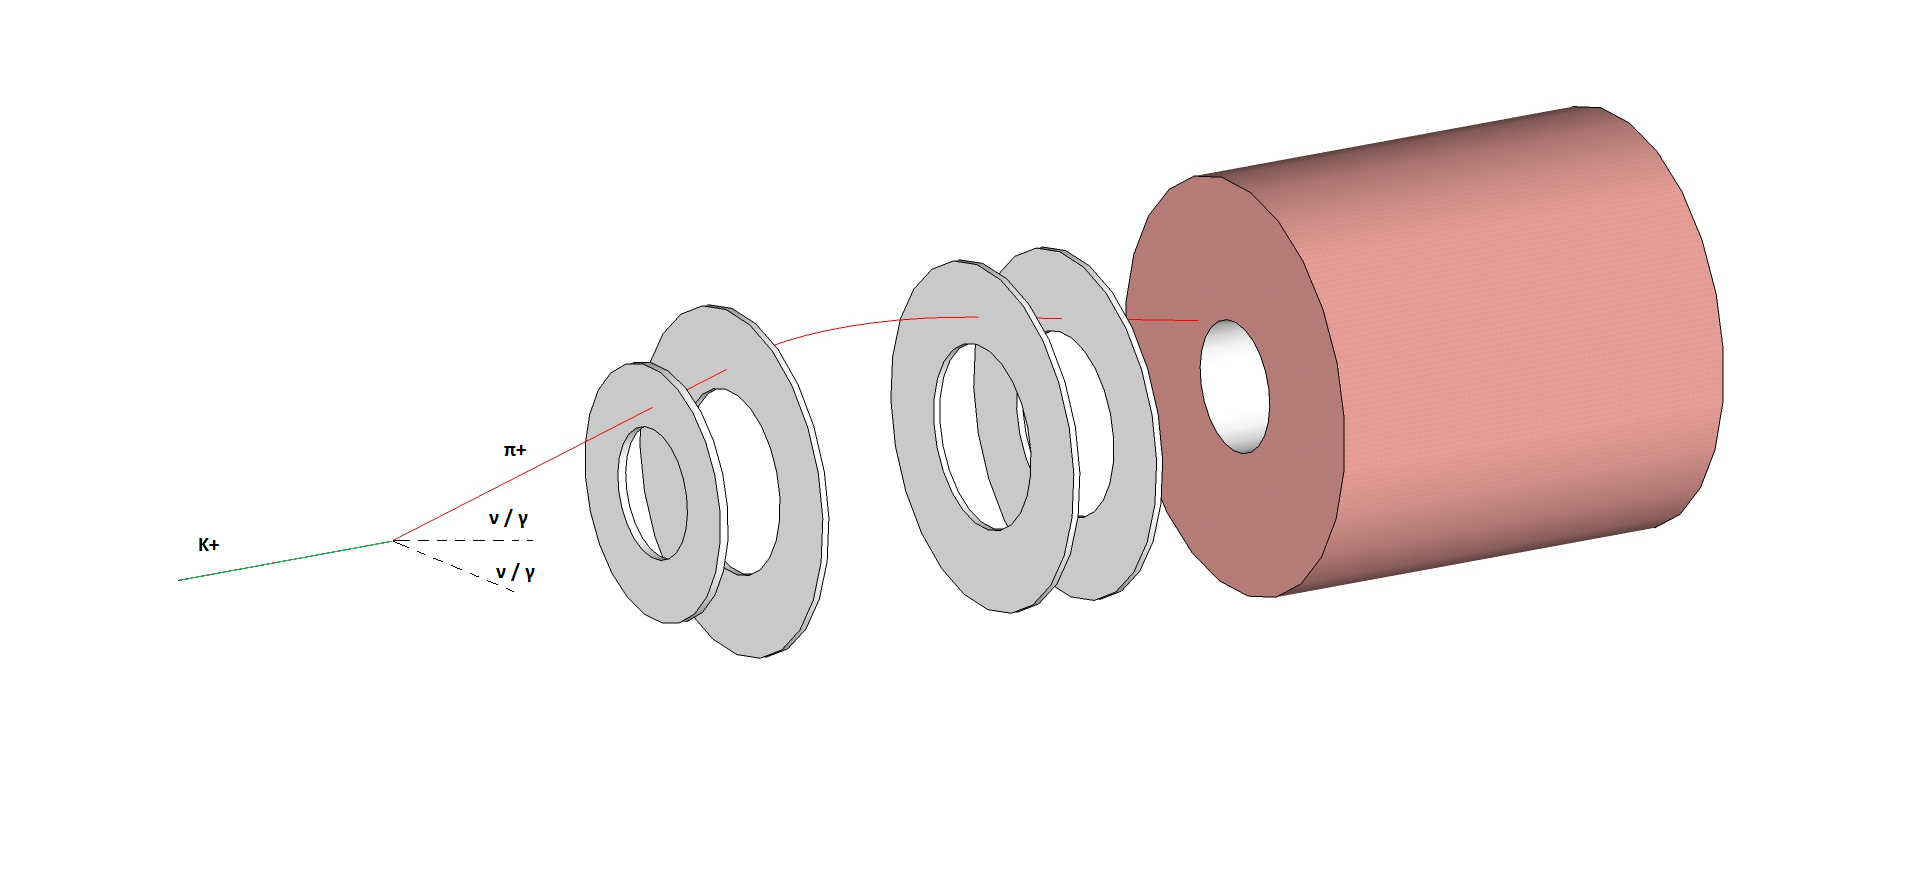
\includegraphics[scale=0.3]{apparato_rare_3d}
\caption{Ricostruzione 3d dell'apparato sperimentale.}
\label{fig:apparato_rare_3d}
\end{figure}

\begin{figure}
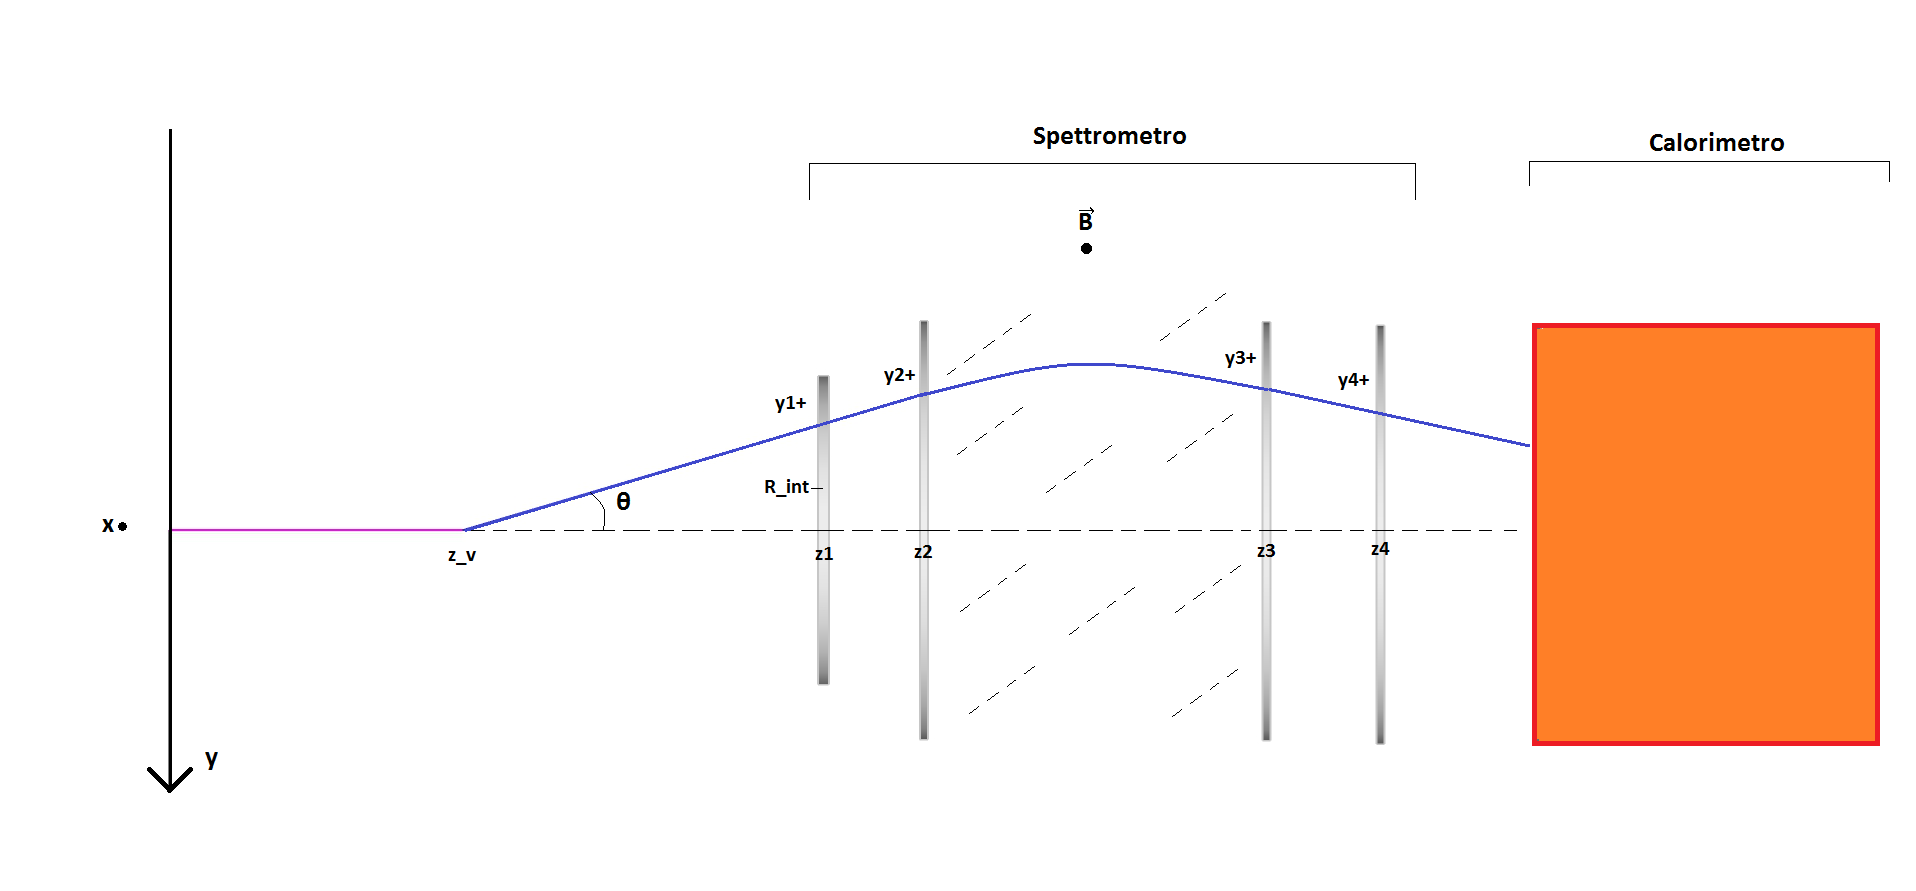
\includegraphics[scale=0.3]{apparato_rare_2d}
\caption{Sezione dell'apparato sperimentale. Il fascio si muove sull'asse z, $z_i$ sono le coordinate dei rivelatori, $R_{int}$ è il loro raggio interno.}
\label{fig:apparato_rare_2d}
\end{figure}

\begin{table}[h!]
\centering
\begin{tabular}{|p{2.5 cm}| p{1 cm}|}
\hline\hline
$p_{beam} (GeV/c)$ & 60 \\
\hline
$\sigma_p (GeV/c)$ & 1 \\
\hline
$<\lambda> (m)$ & 450 \\
\hline
$z_1 (m)$ & 100 \\
\hline
$z_2 (m)$ & 110 \\
\hline
$z_3 (m)$ & 120 \\
\hline
$z_4 (m)$ & 130 \\
\hline
$R_{int,1} (m)$ & 0.1 \\
\hline
$R_{ext,1} (m)$ & 1.25 \\
\hline
$R_{int,2} (m)$ & 0.1 \\
\hline
$R_{ext,2} (m)$ & 1.38 \\
\hline
$R_{int,3} (m)$ & 0.1 \\
\hline
$R_{ext,3} (m)$ & 1.5 \\
\hline
$R_{int,4} (m)$ & 0.1 \\
\hline
$R_{ext,4} (m)$ & 1.8 \\
\hline
$p_{kick} (GeV/c)$ & 0.2 \\
\hline
$\alpha_E$ & 0.2 \\
\hline \hline
\end{tabular}
\caption{Tabella riassuntiva delle caratteristiche dell'apparato sperimentale. $\sigma_x$ è la risoluzione spaziale spettrometro nelle due coordinate misurate, mentre per il calorimetro vale $\sigma_E/E = \alpha_E/\sqrt{E(GeV)}$, $p_{beam}$ è l'impulso del fascio, $\sigma_{beam}$ la sua larghezza, $<\lambda>$ è la lunghezza media di decadimento del $K^+$, $p_{kick}$ il valore del kick del campo magnetico. I calcoli dei valori dei raggi dei piani dello spettrometro sono riportati in sez.\ref{sec:detector}.}
\label{tab:apparato}
\end{table}

Il campo magnetico simulato vale $B = 1.34\ T$, giace sull'asse x ed è confinato in una zona di lunghezza $\Delta L = 0.50\ m$.

\newpage

\section{Struttura del codice} \label{sec:struttura}
Il codice per questa simulazione è stato scritto in C++ utilizzando alcune librerie ROOT per il salvataggio e la visualizzazione dei dati. 
La struttura scelta consiste in tre moduli che lavorano in sequenza, utilizzando l'output del modulo precedente come input e producendo un output e fa uso della classe ROOT \textit{TNtupleD} per il salvataggio dei dati in forma di evento. Questa struttura è ripetuta in modo identico per i due canali di decadimento. I risultati ottenuti per i due canali vengono infine messi a confronto per cercare il miglior taglio degli eventi per una data configurazione sperimentale. In fig.\ref{fig:structure} è mostrato un diagramma che schematizza la struttura del codice. 

\begin{figure}
\begin{center}
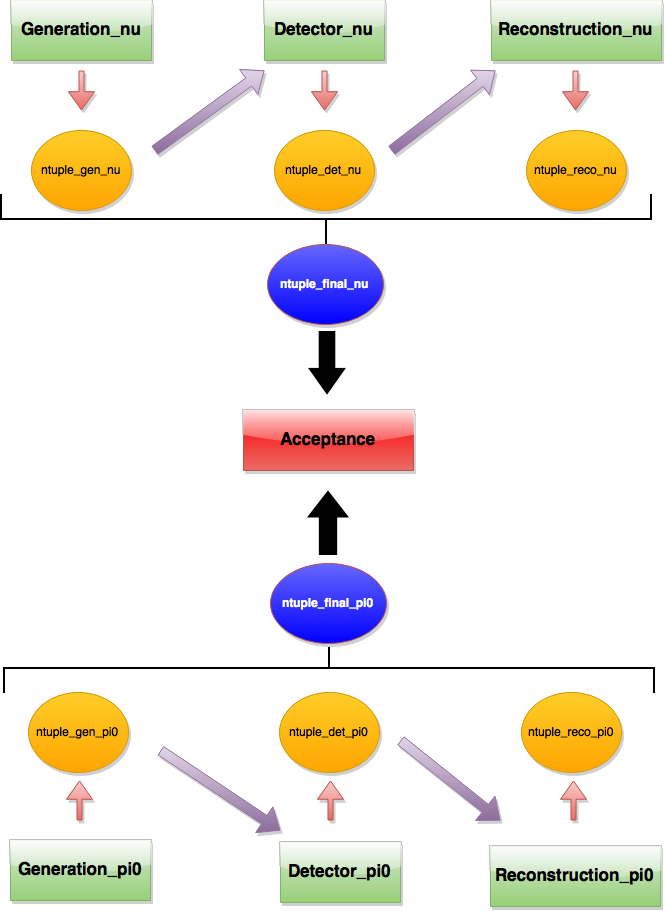
\includegraphics[scale=0.4]{structure_rare}
\caption{Diagramma di flusso della struttura del codice.}
\label{fig:structure}
\end{center}
\end{figure}

I moduli svolgono le seguenti funzioni: \\
\begin{itemize}
\item \textbf{\textit{Generation:}} si occupa della generazione dell'evento. Fa uso della classe ROOT \textit{TGenPhaseSpace} con alcune modifiche apportate nella classe derivata \textit{FGenPhaseSpace}. Produce in uscita il file \textit{ntuple\_gen}.\\
\item \textbf{\textit{Detector:}} si occupa di calcolare i punti di passaggio del $\pi^+$ nello spettrometro, di effettuarne uno smeering e di generare la risposta del calorimetro. Utilizza come input gli eventi generati contenuti in \textit{ntuple\_gen} e produce il file \textit{ntuple\_det}.\\
\item \textbf{\textit{Reconstruction:}} effettua un fit cinematico dell'evento (usando la classe \textit{IterKinFitP}, già usata in una simulazione precedente\cite{spettrometro}) e ne ricostruisce il vertice e l'impulso, nonché la massa mancante, che sarà importante per la scelta dei tagli. Utilizza come input le misure del rivelatore contenute in \textit{ntuple\_det} e produce in output il file \textit{ntuple\_reco} contenente le misure migliorate, la posizione del vertice, l'impulso, la massa mancante e il $\chi^2$ del fit cinematico.\\
\item \textbf{\textit{Acceptance:}} Una volta unite le ntuple dei due canali di decadimento, calcola l'accettanza per i due canali in funzione dei tagli effettuati, nonché la varianza dello stimatore del branching ratio (sez.\ref{sec:acceptance}).
\end{itemize}

La loro funzionalità è descritta nel dettaglio nelle seguenti sezioni.

\newpage

\section{Generazione dell'evento} \label{sec:generation}
Il modulo di generazione fa uso della classe ROOT \textit{TGenPhaseSpace}. Questa classe implementa un algoritmo per generare eventi a molti corpi con spazio delle fasi uniforme come catene di decadimenti a due corpi. L'algoritmo produce eventi \textit{pesati}, che hanno il vantaggio di essere generati in maniera più veloce ma alcune complicazioni pratiche come quella di dover tenere in memoria, evento per evento, il suo peso per tutti e tre i moduli. Si è deciso di scrivere una classe derivata, chiamata \textit{FGenPhaseSpace}, in cui le funzionalità della classe madre vengono preservate ma si aggiunge la possibilità di generare eventi senza peso. Questo è stato realizzato sostanzialmente normalizzando il peso dell'evento al peso massimo di tale classe di eventi e accettando ogni evento con probabilità uguale a tale peso normalizzato. In fig.\ref{fig:gen_E_beam} - \ref{fig:gen_miss} sono mostrate le distribuzioni di alcune quantità rilevanti degli eventi. Si indica da ora in avanti con \textit{N} il decadimento a due corpi e con \textit{R} quello raro a tre corpi. 

\begin{figure}
\begin{center}
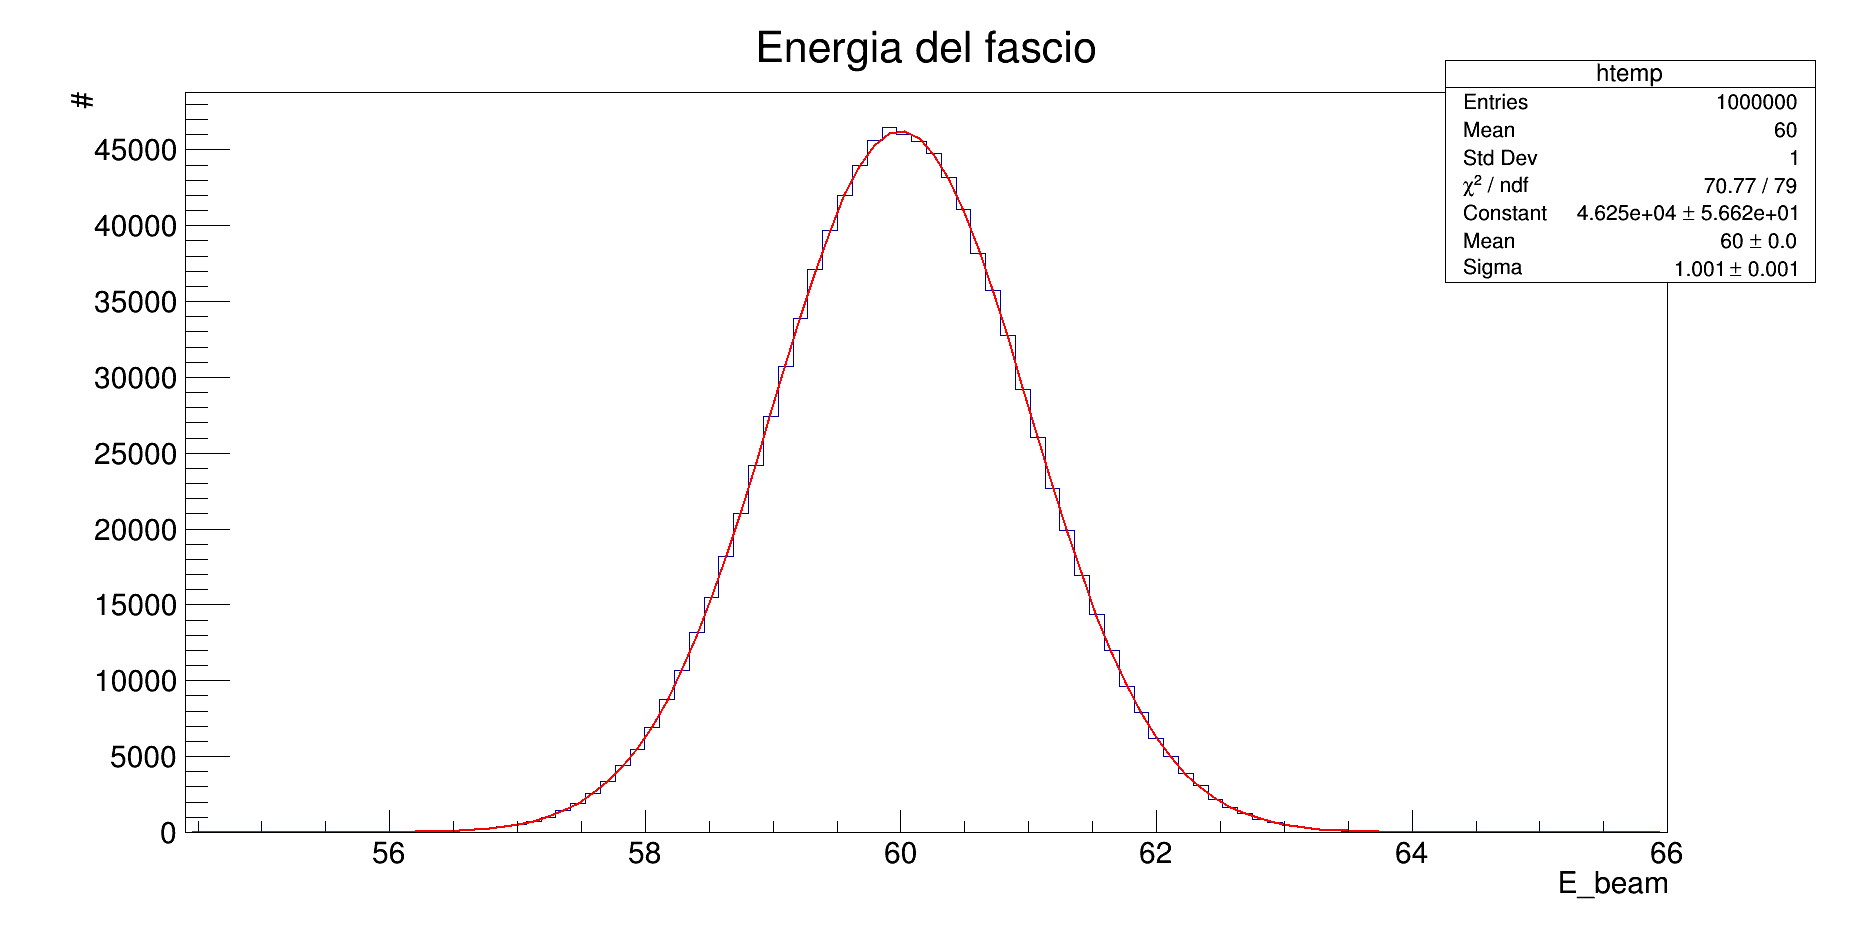
\includegraphics[scale=0.25]{gen_E_beam}
\caption{Energia del fascio.}
\label{fig:gen_E_beam}
\end{center}
\end{figure}

\begin{figure}
\begin{center}
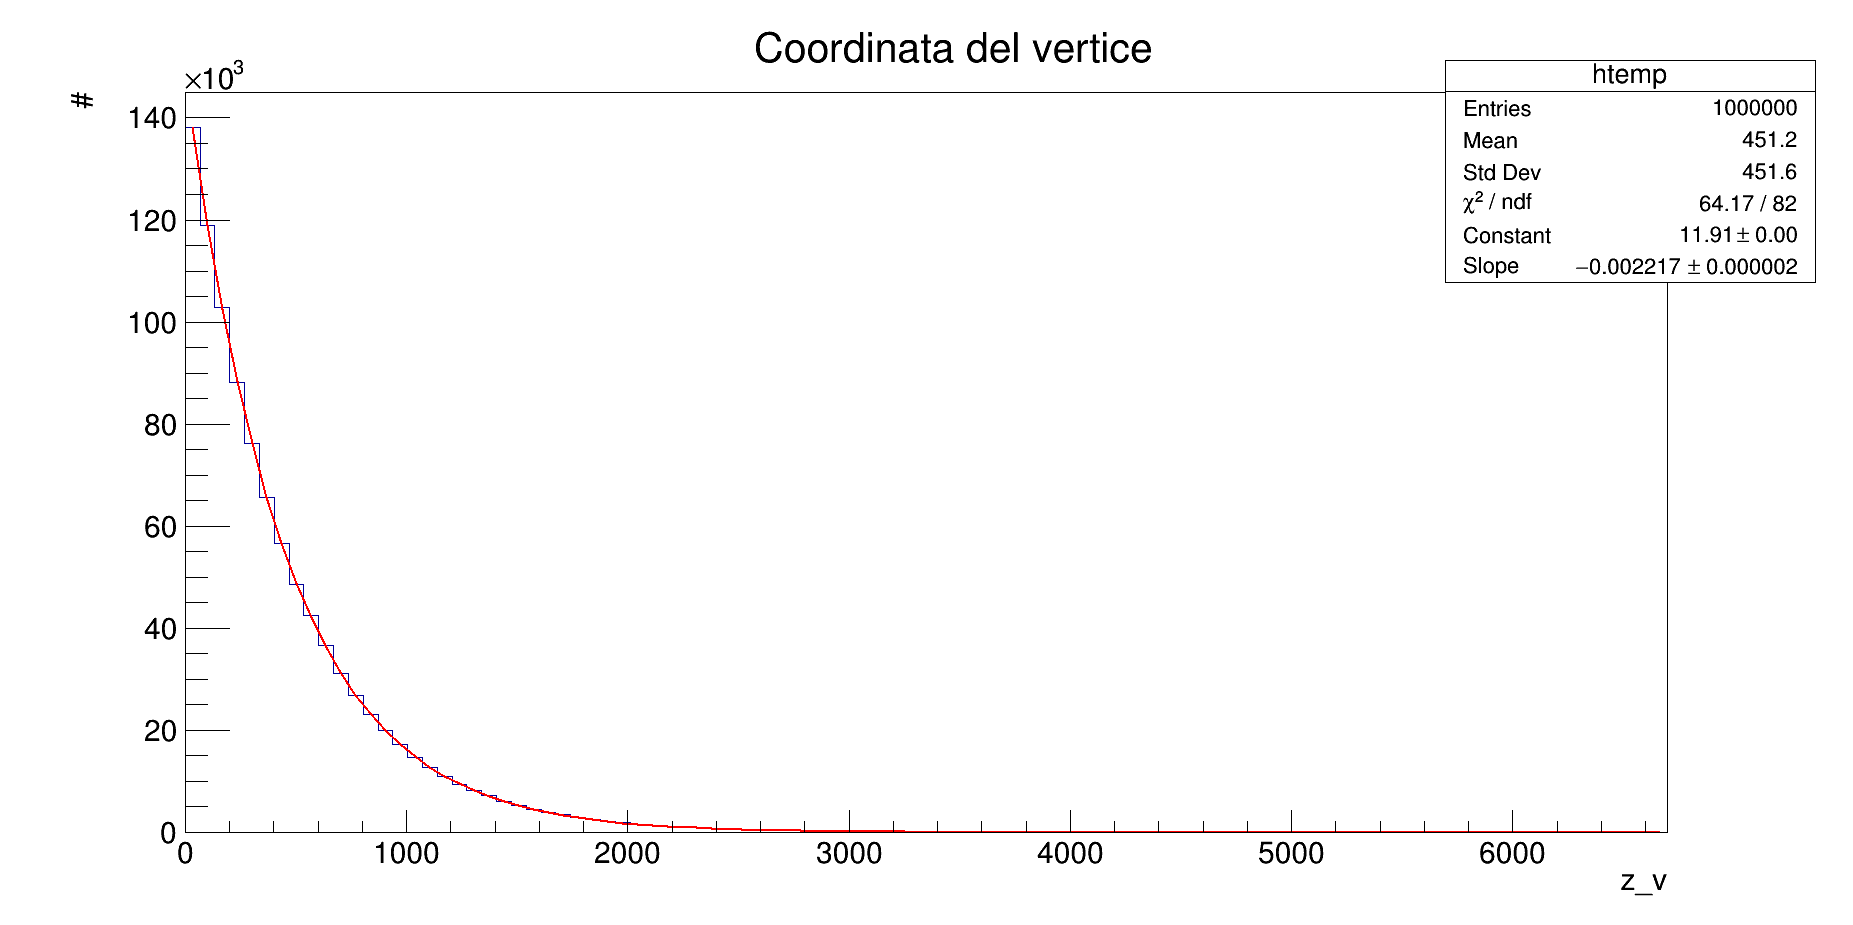
\includegraphics[scale=0.25]{gen_z}
\caption{Coordinata del vertice.}
\label{fig:gen_z}
\end{center}
\end{figure}

\begin{figure}
\begin{center}
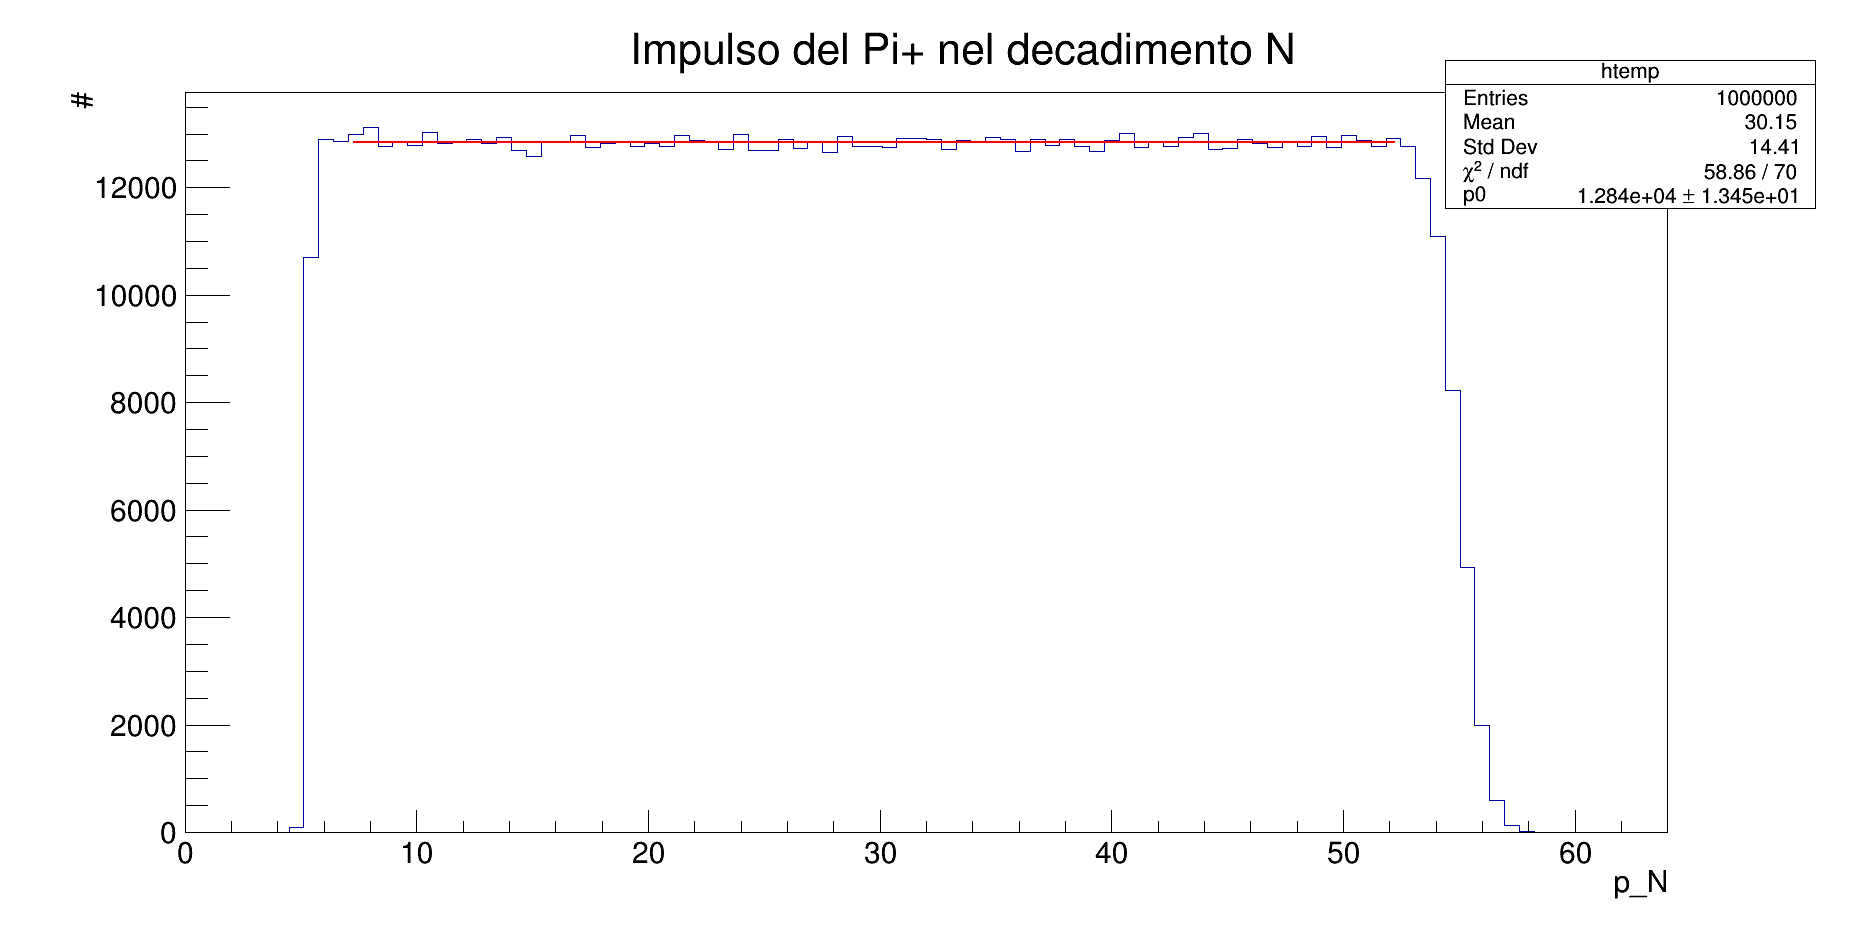
\includegraphics[scale=0.25]{gen_p_N}
\caption{Impulso del $\pi^+$ nel decadimento a due corpi.}
\label{fig:gen_p_N}
\end{center}
\end{figure}

\begin{figure}
\begin{center}
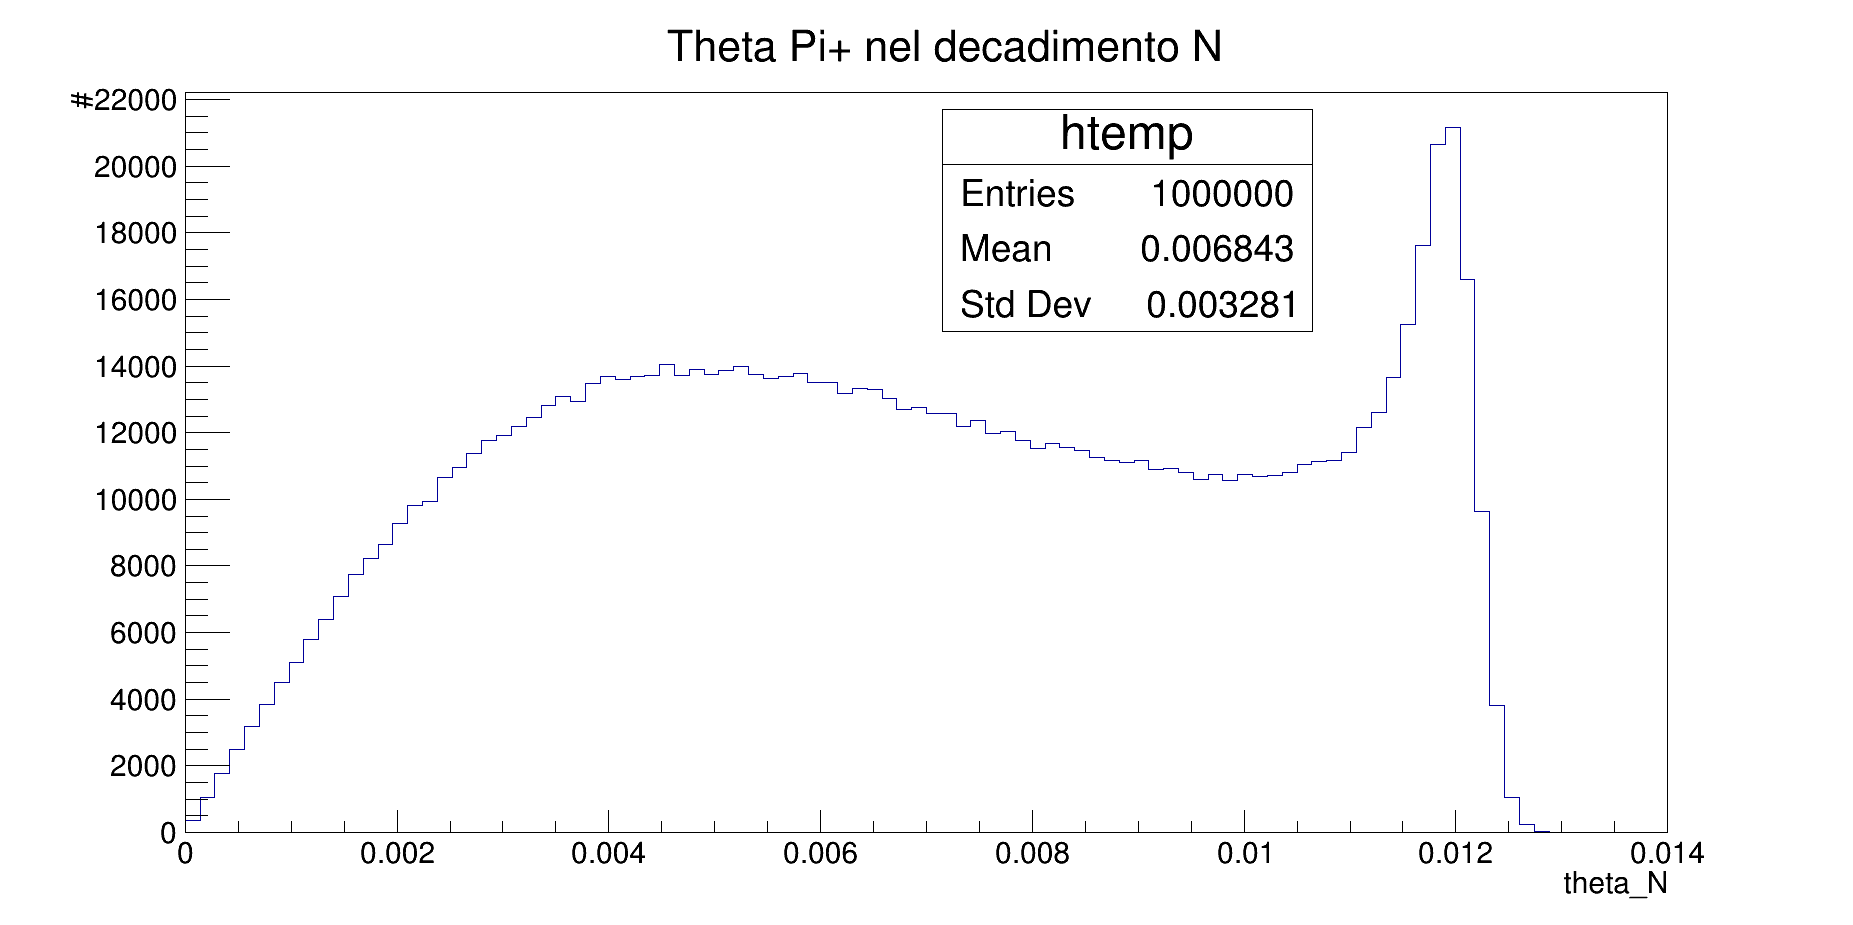
\includegraphics[scale=0.25]{gen_theta_N}
\caption{$\theta$ del $\pi^+$ nel decadimento a due corpi.}
\label{fig:gen_theta_N}
\end{center}
\end{figure}

\begin{figure}
\begin{center}
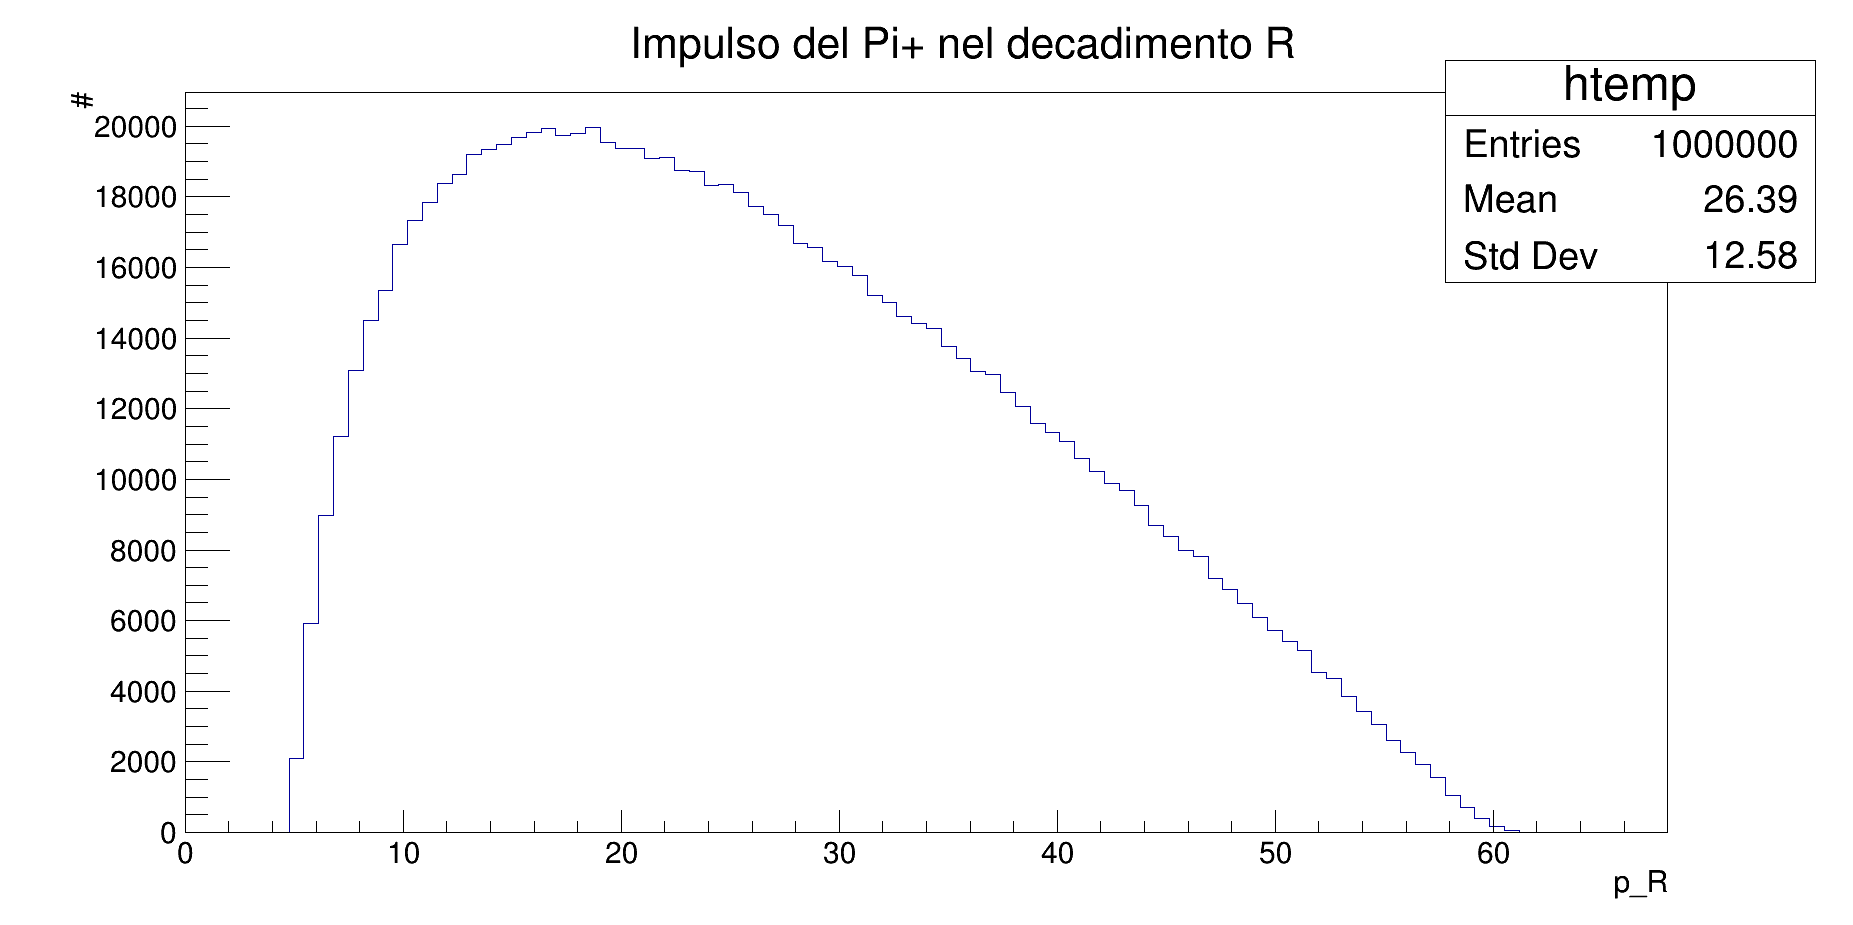
\includegraphics[scale=0.25]{gen_p_R}
\caption{Impulso del $\pi^+$ nel decadimento a tre corpi.}
\label{fig:gen_p_R}
\end{center}
\end{figure}

\begin{figure}
\begin{center}
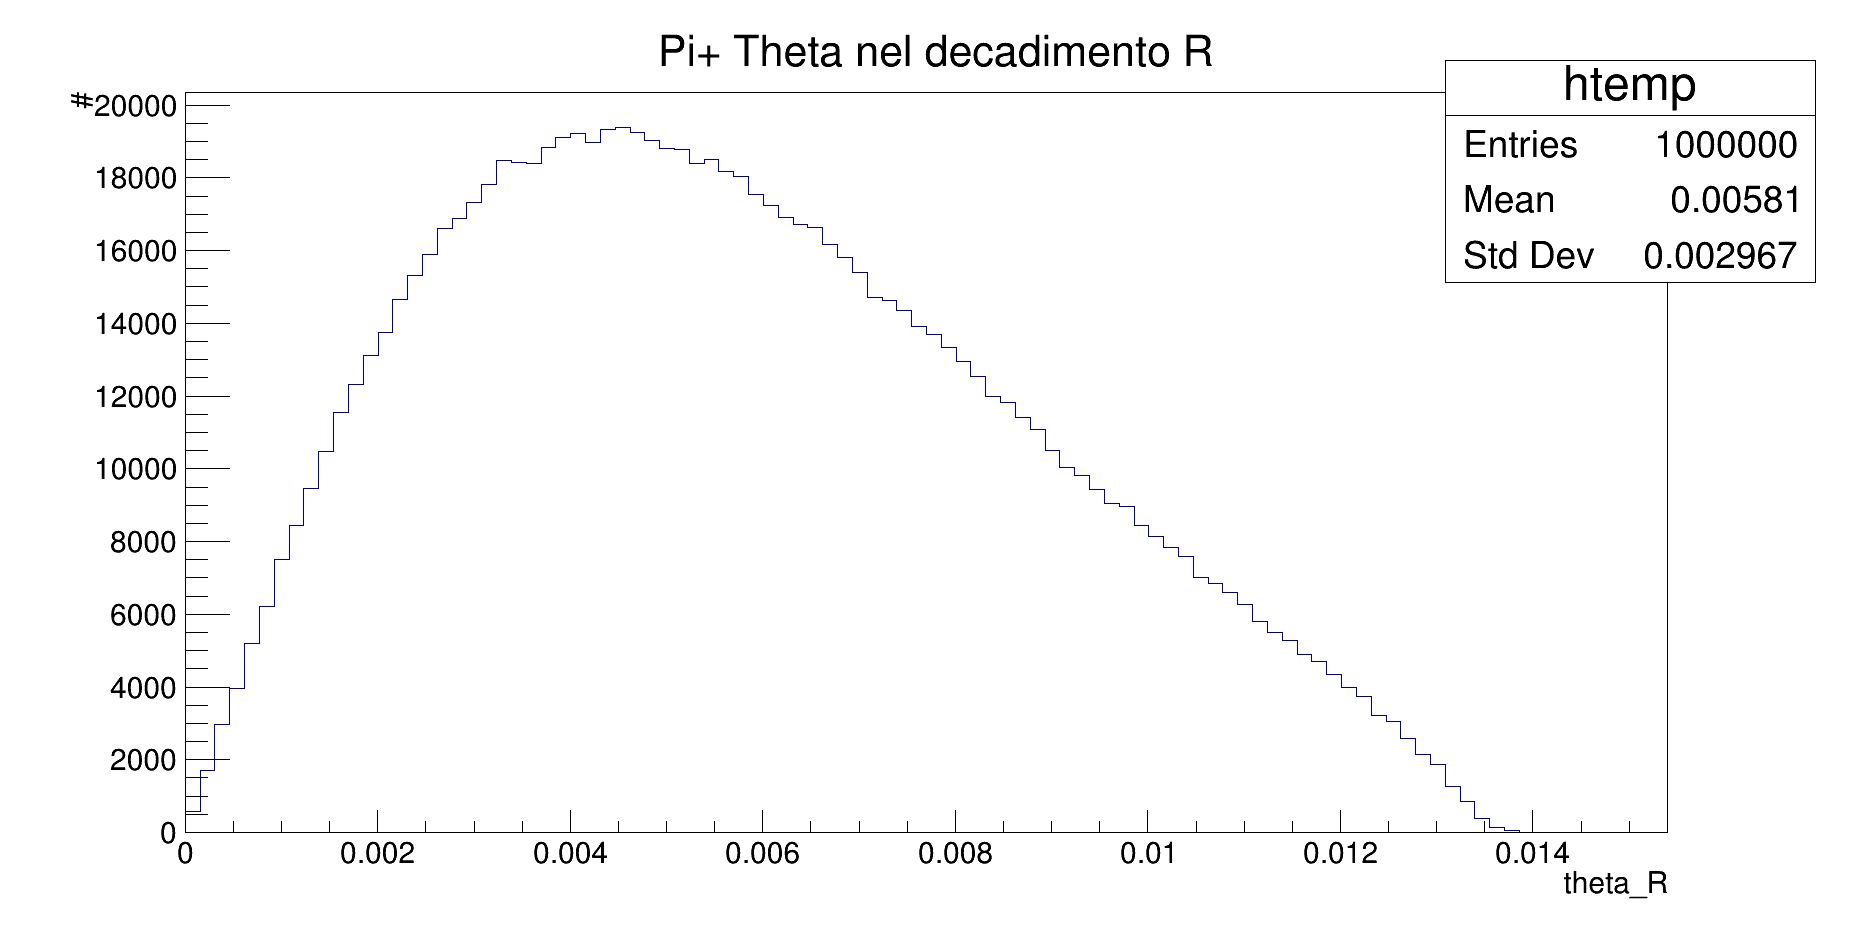
\includegraphics[scale=0.25]{gen_theta_R}
\caption{$\theta$ del $\pi^+$ nel decadimento a tre corpi.}
\label{fig:gen_theta_R}
\end{center}
\end{figure}

\begin{figure}
\begin{center}
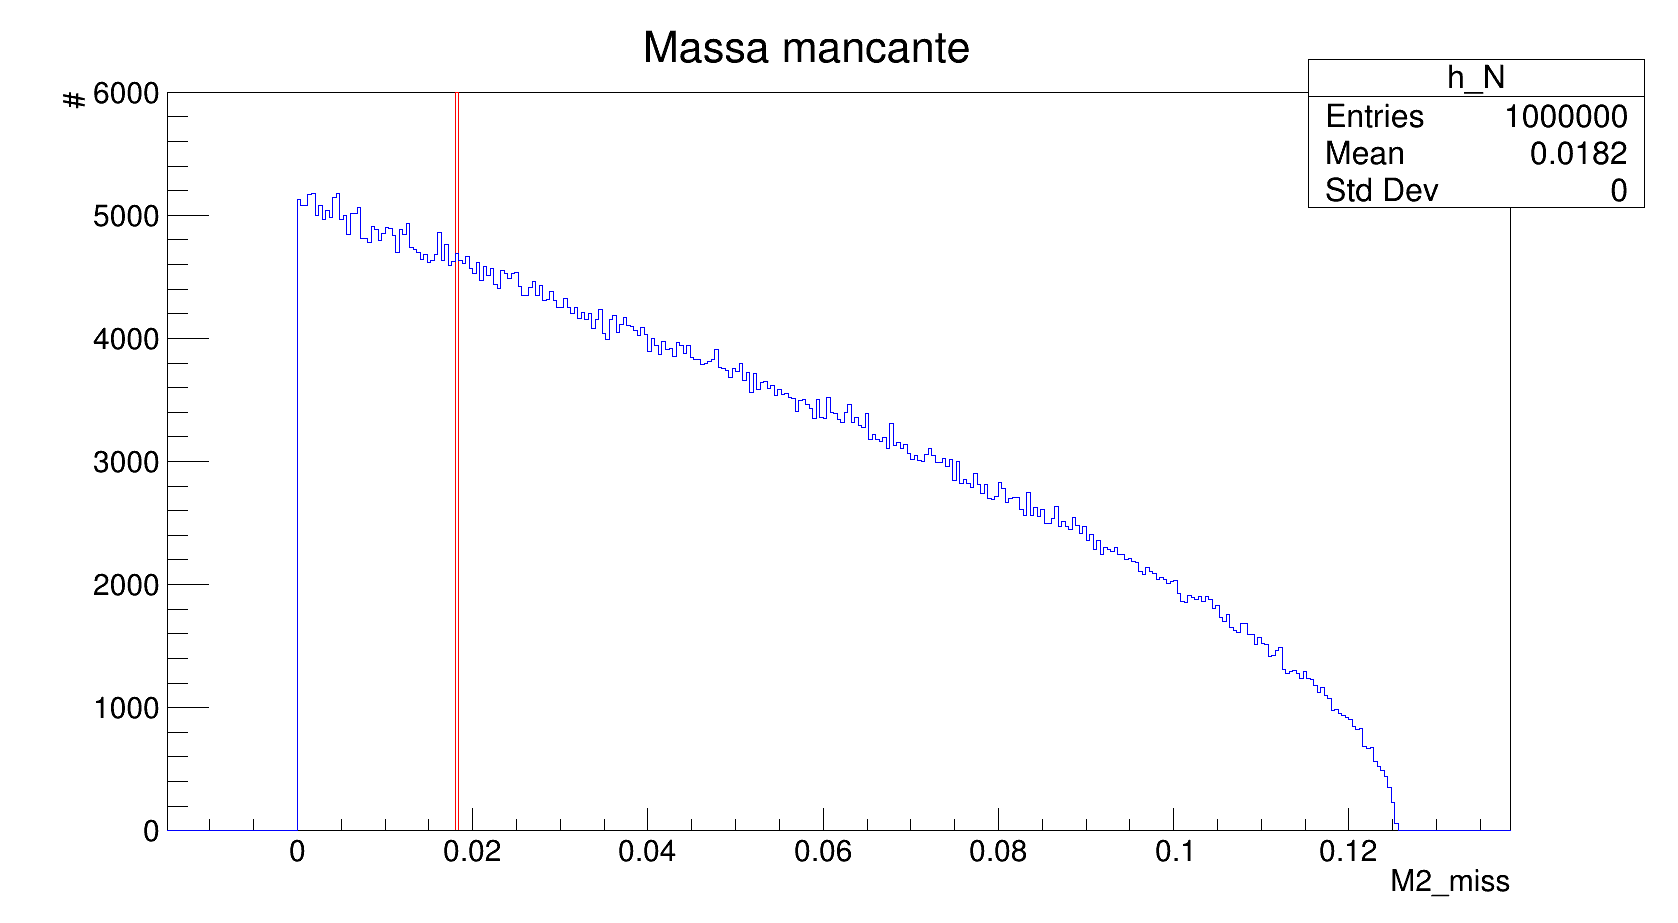
\includegraphics[scale=0.25]{gen_miss}
\caption{Distribuzione della massa mancante nei due canali di decadimento, in rosso in quello a due corpi, in blu quello a tre.}
\label{fig:gen_miss}
\end{center}
\end{figure}

Vediamo che la principale differenza tra i due canali di decadimento risiede nella distribuzione della massa mancante, definita come: \\
$$
M^2_{miss} = (K^{\mu} - \pi^{\mu})^2 = M^2_K +  M^2_{\pi^+} - 2E_K E_\pi + 2 p_K p_\pi \cos(\theta)
$$

Nel caso del decadimento a due corpi questa quantità è distribuita come una $\delta$, mentre in quello a tre corpi ha una distribuzione continua. 
In realtà un'altra differenza si può riscontrare nell'angolo e nell'impulso massimo dei due canali di decadimento, ma si tratta di una piccola differenza difficilmente sfruttabile se non con un apparato a risoluzione molto elevata e a scapito dell'accettanza. 


\section{Simulazione della risposta dei rivelatori} \label{sec:detector}
Il modulo \textit{Detector} si occupa prima di tutto di calcolare i punti di passaggio reali della particella nello spettrometro. Per fare questo è stata seguita la stessa procedura già utilizzata in un lavoro precedente\cite{spettrometro} sfruttando i dati provenienti da \textit{ntuple\_gen}. Sono stati quindi calcolati i punti di passaggio utilizzando l'approssimazione di kick del magnete, giustificata dal fatto che $p_{kick} = 0.2\ GeV/c << p_{min} = 5\ GeV/c$. Uno smeering gaussiano di larghezza $\sigma_x$ è stato poi applicato ai punti per produrre i dati sperimentali (vedi tab.\ref{tab:apparato}, sez.\ref{sec:apparato}). La risposta del calorimetro è stata anch'essa supposta gaussiana, con una larghezza dipendente dall'energia e uguale a $\sigma_E (GeV) = 20\% \sqrt{E(GeV)}$. I risultati sono stati salvati in \textit{ntuple\_det}.

Con questi dati è anche possibile calcolare i raggi interni ed esterni di tutti i rivelatori dello spettrometro in modo da massimizzare l'accettanza. Fissato infatti $R_{int, 1} = 0.1\ m$ per il fascio, sono stati tagliati gli eventi con $\sqrt{x^2+y^2} < 0.1\ m$ su tutti i piani e misurata la distribuzione delle quantità $\sqrt{x^2 + y^2}$ su ogni rivelatore. Il minimo di questa quantità determina il raggio interno, il massimo il raggio esterno. I risultati sono quelli riportati in tab.\ref{tab:apparato}. Essendo inoltre $c\tau_{\pi^+} \approx 1\ m$ e $\gamma_{\pi, min} \approx 36$, è stato necessario tagliare gli eventi in cui il $\pi^+$ decade prima di attraversare l'ultimo rivelatore.

\section{Ricostruzione dell'evento} \label{sec:reconstruction}
Per la ricostruzione dell'evento è stato scelto un fit cinematico iterativo, implementato nella classe \textit{IterKinFitP}, descritta nel dettaglio in \cite{spettrometro}. Il fit cinematico è stato basato su 9 quantità misurate (le 8 coordinate dallo spettrometro e la misura calorimetrica), di 7 vincoli e 2 parametri non misurati ($z_v$, ovvero posizione del vertice $p$, impulso). I vincoli sfruttati sono stati: 

\begin{equation}
x_1 (z_{2,3,4} - z_v) - x_{2,3,4} (z_1 - z_v) = 0
\end{equation}

\begin{equation}
y_1 (z_{2} - z_v) - y_{2} (z_1 - z_v) = 0
\end{equation}

\begin{equation}
y_3 - y_1 - (y_2-y_1)\frac{z_3-z_1}{z_2-z_1} - \frac{z_3-z_2}{2} \frac{p_k}{p} = 0
\label{eq:curvaturay3}
\end{equation}

\begin{equation}
\frac{y_4-y_3}{z_4-z_3} - \frac{y_2-y_1}{z_2-z_1} - \frac{p_k}{p} = 0
\end{equation}

\begin{equation}
E^2 - p^2 - m_\pi^2 = 0
\end{equation}

Le prime due equazioni rappresentano la linearità della traccia e il fatto che essa sia generata da un vertice comune sull'asse z. Per l'asse x si tratta di 3 vincoli perché questa coordinata non viene (nell'approssimazione di kick) influenzata dal campo magnetico. Per l'asse y si tratta invece di un solo vincolo per il motivo contrario. La terza equazione invece origina dal fatto che le tracce entrante e quella uscente si intersechino nel punto medio tra i rivelatori centrali. La quarta è il vincolo di curvatura dovuto alla presenza del campo magnetico; la quinta, infine, è la condizione di mass shell. In sez.\ref{sec:grafici} sono mostrati i risultati della ricostruzione (fig.\ref{fig:reco_x1_N} - fig.\ref{fig:reco_miss_norm}).


\section{Accettanza} \label{sec:acceptance}
\subsection{Livello di rigetto del fondo} \label{subsec:rejection}
L'ultimo modulo (\textit{Acceptance}) raccoglie i dati provenienti dalle ricostruzioni degli eventi relativi ai due canali di decadimento e si occupa di cercare il taglio che permette di misurare il branching ratio del processo in esame con una certa precisione nella maniere più efficiente possibile (ovvero minimizzando il tempo di misura necessario per ottenere tale precisione). \'E quindi necessario svolgere dei calcoli per trovare uno stimatore del branching ratio e la sua varianza, riportati nel dettaglio in sez.\ref{sec:calcoli}. Si ricava la stima del tempo di misura:

$$
t = \frac{1}{R \alpha^2 BR_R^2} (\mu \cdot Var(\widehat{BR_R}))
$$

con \textit{R} uguale al rate di $K^+$, $\alpha$ la precisione relativa desiderata per la misura del branching ratio, $\mu \cdot Var(\widehat{BR_R})$ la quantità ricavata dalla simulazione: 

\begin{equation}
\mu \cdot Var(\widehat{BR_R}) = \frac{a_{N,cut}a_{N,geom}BR_N + a_{R,cut}a_{R,geom}BR_R}{(a_{R,cut}a_{R,geom})^2}
\end{equation}

dove $a$ sono le accettanze di taglio (cut) e geometriche (geom) relative ai decadimenti nei canali $\pi^+ \pi^0$ (N) e $\pi^+ \nu \bar{\nu}$ (R).

In questo valore appare la quantità da misurare $BR_R$: per progettare l'esperimento è chiaramente necessario avere una stima di questa quantità. Come scritto in sez.\ref{sec:intro}, un calcolo teorico fornisce un valore con un'incertezza di qualche percento\cite{br teorico}. Nella simulazione esso è stato fissato al valore $BR_R = 10^{-10}$.

Per quanto riguarda R, per usare un valore ragionevole è stato scelto quello dell'esperimento NA62\cite{NA62 flux}:
$$
R = 4.5 \cdot 10^{12} decays/y = 1.43 \cdot 10^5 decays/s
$$

Fissando invece $\alpha = 10\%$ abbiamo:

$$
t = (\mu \cdot Var(\widehat{BR_R})) \cdot 2.2 \cdot 10^9\ y
$$

Per ridurre i tempi di misura è necessario trovare il taglio che minimizzi la quantità $\mu \cdot Var(\widehat{BR_R})$. 
La selezione è della forma $M^2_{miss} > M^2_c$, dove $M^2_c$ è la massa mancante e $M^2_c$ il valore critico scelto per la selezione. Fissata la configurazione dell'apparato sperimentale, le accettanze geometriche sono fissate e le accettanze di taglio dipendono da $M^2_c$. Per valori piccoli di $M^2_c$ le accettanze dei due canali saranno confrontabili e, a causa del valore estremamente piccolo di $BR_R$, il numeratore di $\mu \cdot Var(\widehat{BR_R})$ sarà dominato dall'accettanza del canale N. Risulta quindi:

$$
t \approx \frac{a_{N, cut} a_{N, geom}}{(a_{R, cut} a_{R, geom})^2}\ 2.2 \cdot 10^9 y
$$

Questa situazione si verifica fino a che $a_{N, cut} a_{N, geom} >> a_{R, cut} a_{R, geom} BR_R$. Se l'accettanza totale del canale R è dell'ordine di $10 \%$ questo significa che la condizione sussiste fino a che 
$$
a_{N, cut} a_{N, geom} >> 10^{-11}
$$

e quindi fino a circa $10^{-10}$.

In questa situazione il tempo di misura decresce con l'aumentare di $M^2_c$ perché tipicamente l'accettanza del canale N diminuisce più rapidamente del quadrato dell'accettanza del canale R.

Quando invece si verifica la situazione inversa in cui l'accettanza totale del canale N è $\lesssim 10^{-12}$ il tempo di misura necessario è:

$$
t \approx \frac{BR_R}{a_{R, cut}a_{R,geom}} 2.2 \cdot 10^9\ y = \frac{1}{a_{R, cut}a_{R,geom}} 0.22\ y
$$

In questa situazione il tempo cresce all'aumentare di $M^2_c$, perché rendere più severo il taglio ha il solo effetto di ridurre la statistica. Ci deve essere quindi un valore di $M^2_c$ intermedio tra queste situazioni in cui il tempo di misura necessario raggiunge un minimo. Minimizzare il tempo di misura equivale, in termini di segnale e rumore, a massimizzare la quantità 
$$
\frac{1}{Rt} \frac{S^2}{S+N} = \frac{(a_{R,geom}a_{R,cut}BR_R)^2}{a_{N,geom}a_{N,cut}BR_N + a_{R,geom}a_{R,cut}BR_R}
$$

indipendente dal tempo, per cui:

$$
t = 2.2\cdot 10^{-11} (Rt \frac{S+N}{S^2})\ y
$$

\subsection{Calcolo dell'accettanza}

La stima dell'accettanza geometrica è effettuata calcolando il rapporto tra il numero di eventi accettati dal sistema e il numero di eventi generati. La stima dell'accettanza di taglio è invece effettuata calcolando il rapporto tra il numero di eventi che superano il taglio e il numero di eventi accettati dal sistema. Per quanto riguarda le accettanze geometriche, con la configurazione descritta in tab.\ref{tab:apparato},sez.\ref{sec:apparato}, risulta:
$$
a_{N, geom} = 0.14781 \pm 0.00035
$$
$$
a_{R, geom} = 0.13983 \pm 0.00035
$$

dove gli errori sono stati stimati tenendo conto che il numero di eventi accettati è distribuito come una binomiale: 
$$
\sigma_a \approx \sqrt{\frac{a(1-a)}{N_{gen}}}
$$

 In fig.\ref{fig:acc_taglio} sono mostrati gli andamenti delle accettanze di taglio per i due canali di decadimento.
 
 \begin{figure}
 \begin{center}
 	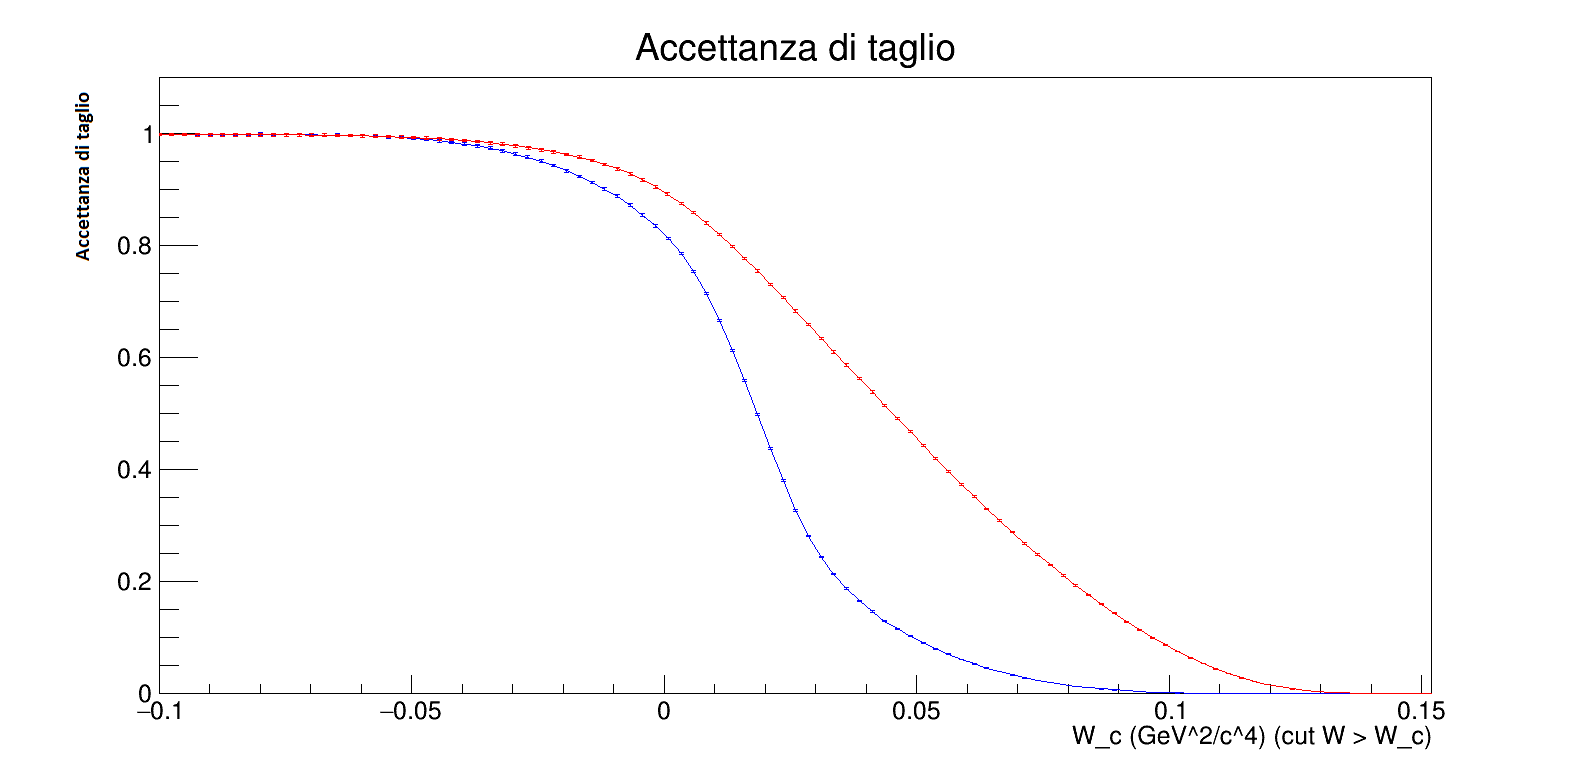
\includegraphics[scale=0.3]{acc_taglio}
 	\caption{Accettanze di taglio per il canale N($\pi^+ \pi^0$, blu) e per quello R($\pi^+ \nu \bar{\nu}$, rosso).}
 	\label{fig:acc_taglio}
 \end{center}
 \end{figure}

In sez.\ref{subsec:rejection} è stato ottenuto che il livello di accettanza richiesto per il fondo è circa $10^{-12}$. Tuttavia, per calcolare tale livello di accettanza è necessario generare un numero di eventi dell'ordine di $10^{12}$, che non è possibile con i mezzi tecnologici a disposizione. Ci sono due possibilità per ovviare a questo problema: 

\begin{itemize}
\item Studiare la gaussianità delle code della distribuzione di massa mancante del fondo.
\item Utilizzare un sistema indipendente di taglio del fondo (Veto, Particle ID...)
\end{itemize}

Per quanto riguarda la \textbf{prima possibilità}, si tratta chiaramente di un'approssimazione perché non è stata riscontrata alcuna indicazione che la distribuzione sia effettivamente gaussiana. Il fit ha portato a un risultato compatibile con una distribuzione gaussiana con significatività del 99\% ($\chi^2/NDF = 29.1/19$) (fig.\ref{fig:reco_miss_N_fit}). Si può calcolare il livello $M^2_c$ oltre il quale la frazione di eventi contenuta è $10^{-12}$ nel modo seguente:

$$
\int_{M^2_c}^{\infty} \frac{1}{\sqrt{2\pi}\sigma} e^{-\frac{(x-\mu)^2}{2\sigma^2}} dx = \frac{1}{2}(1 - erf(\frac{M^2_c-\mu}{\sqrt{2}\sigma})) = 10^{-12}
$$
$$
M^2_c - \mu = 7\sigma
$$

 \begin{figure}
 \begin{center}
 	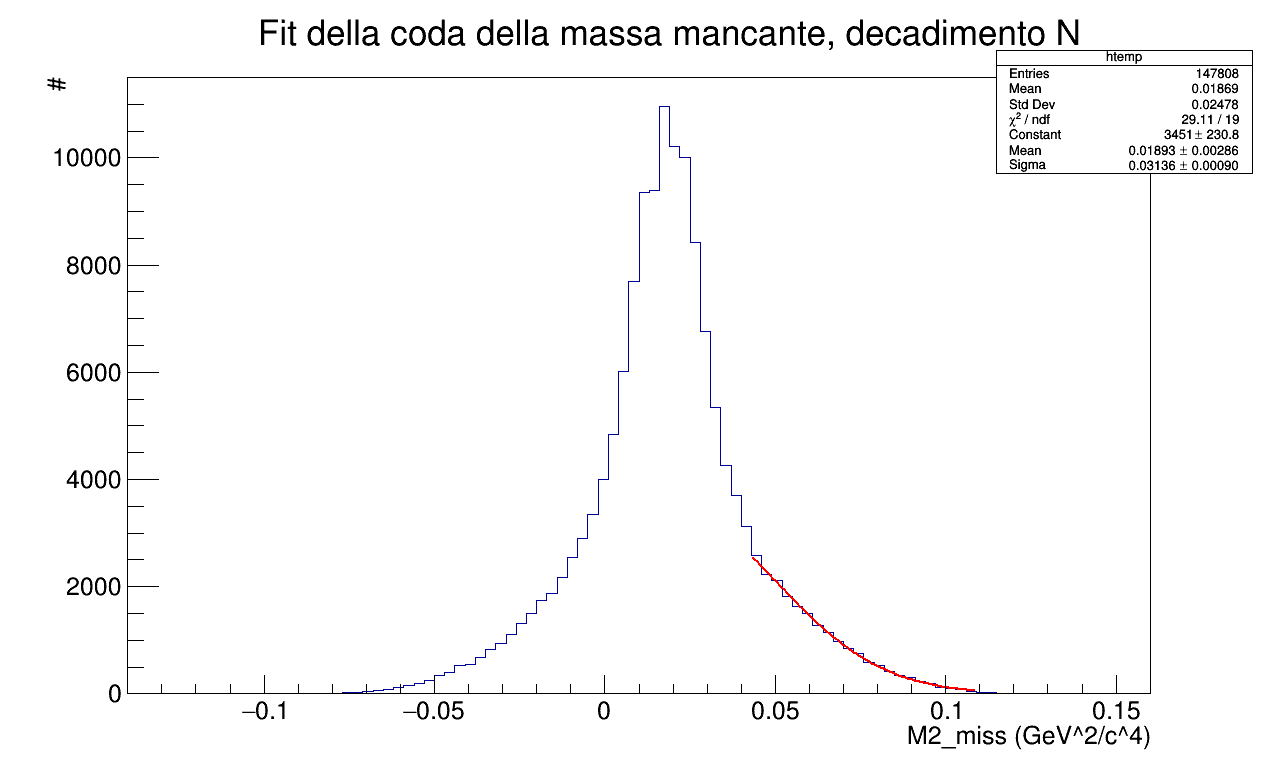
\includegraphics[scale=0.25]{reco_miss_N_fit}
 	\caption{Fit gaussiano della coda della distribuzione di massa mancante.}
 	\label{fig:reco_miss_N_fit}
 \end{center}
 \end{figure}

In realtà, siccome si tratta di un'approssimazione, è più sicuro moltiplicare il coefficiente della $\sigma$ per un \textit{safety factor}, che scegliamo valere 3. Risulta quindi: 
$$
M^2_c = 0.68\ GeV^2/c^4
$$ 

Come si può vedere anche da fig.\ref{fig:reco_miss_norm}, si tratta di un valore al quale anche il segnale è soppresso (fuori scala nella figura).

La \textbf{seconda possibilità} è più pulita da un punto di vista statistico e prevede l'uso di un apparato per la rivelazione dei fotoni. Supponiamo ad esempio che questo abbia un'efficienza di $1 - 10^{-8}$ e per semplicità supponiamo che abbia una copertura angolare del 100\%. L'accettanza totale del canale $\pi^+ \pi^0$ è dunque scalata di un fattore $10^{-8}$. In fig.\ref{fig:acc_taglio_veto}, \ref{fig:acc_s2}, \ref{fig:acc_snratio} sono mostrati i profili delle accettanze per i due canali, la quantità $\frac{1}{Rt} \frac{S^2}{S+N}$ (che si è vista in sez.\ref{subsec:rejection} essere legata al tempo di misura necessario) e il rapporto segnale rumore $S/N$ in funzione del valore del taglio $M^2_c$.

 \begin{figure}
 \begin{center}
 	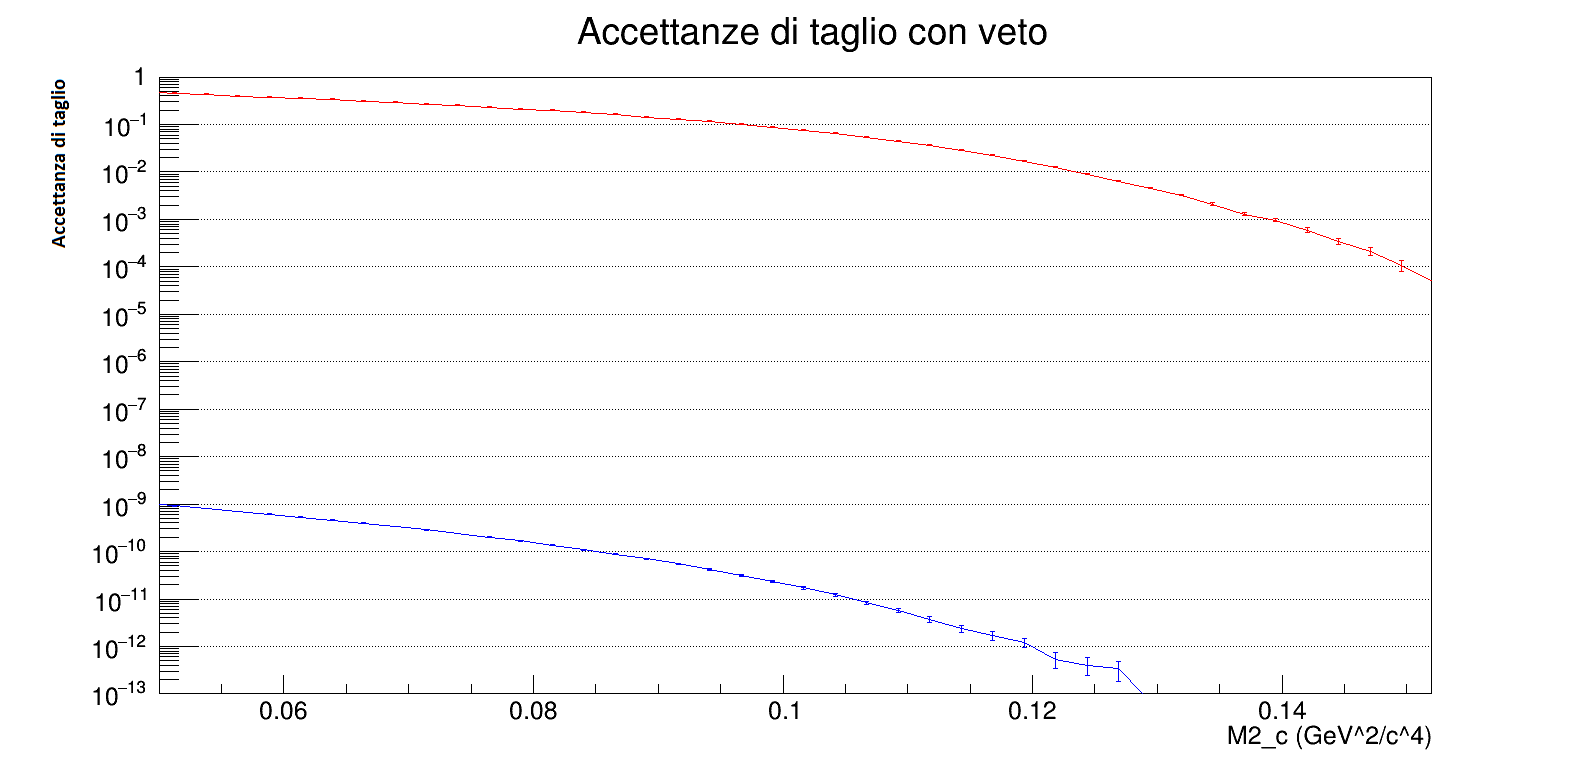
\includegraphics[scale=0.3]{acc_taglio_veto}
 	\caption{Grafico in scala logaritmica delle accettanze dei due canali con veto per i fotoni del $\pi^0$.}
 	\label{fig:acc_taglio_veto}
 \end{center}
 \end{figure}

 \begin{figure}
 \begin{center}
 	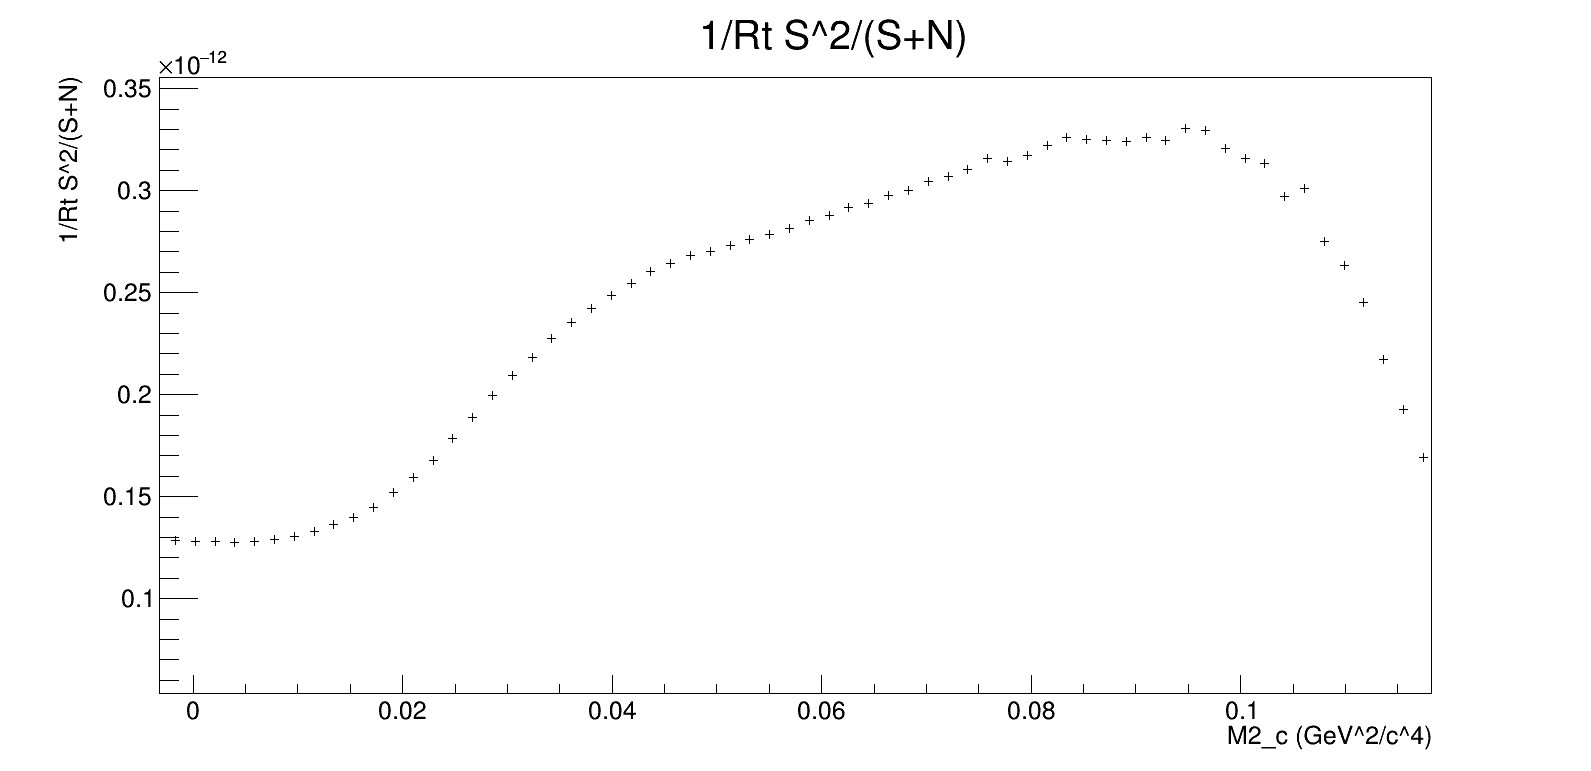
\includegraphics[scale=0.25]{acc_s2}
 	\caption{Grafico di $\frac{1}{Rt} \frac{S^2}{S+N}$.}
 	\label{fig:acc_s2}
 \end{center}
 \end{figure}
 
  \begin{figure}
 \begin{center}
 	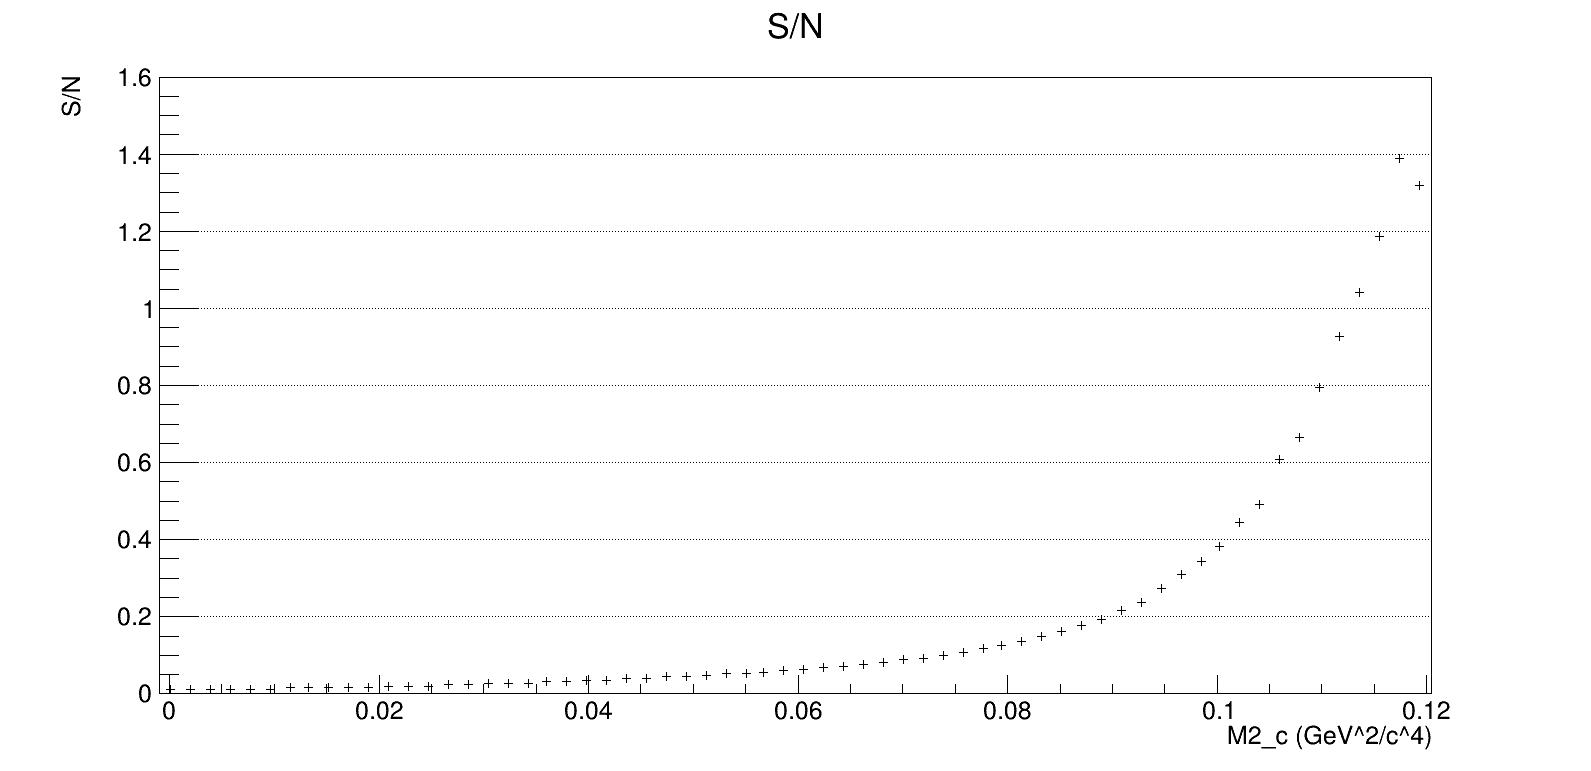
\includegraphics[scale=0.25]{acc_sn}
 	\caption{Grafico del rapporto segnale-rumore $S/N$.}
 	\label{fig:acc_snratio}
 \end{center}
 \end{figure}

Risulta che il taglio migliore è 
$$
M^2_{reco} > 0.095\ GeV^2/c^4
$$

e come stima del tempo di misura necessario:
$$
t \approx 60\ y
$$

\newpage

\section{Conclusioni} \label{sec:conclusioni}

Il tempo di misura trovato rende l'esperimento impossibile da realizzare con questa configurazione sperimentale. Notiamo che il tempo di misura minimo si ottiene quando l'accettanza del fondo è trascurabile e l'accettanza degli eventi di segnale è $100\%$ e vale $0.22\ y$, che sarebbe invece accettabile. Ci sono vari modi per migliorare l'accettanza degli eventi di segnale:

\begin{itemize}
\item \textit{Ingrandire l'esperimento:} questo risulta in un miglioramento della parte geometrica dell'accettanza, nonché in un miglioramento della risoluzione dello spettrometro.
\item \textit{Migliorare la risoluzione in massa mancante:} usare rivelatori più accurati porterebbe a ridurre il valore di $M^2_c$, per cui l'accettanza degli eventi di segnale aumenterebbe.
\item \textit{Migliorare il sistema di veto:} stesso effetto del caso precedente.
\end{itemize}

Tra i limiti della simulazione si trovano:
\begin{itemize}
\item \textit{Elemento di matrice del decadimento $K^+ \rightarrow \pi^+ \nu \bar{\nu}$:} non considerato.
\item \textit{Fondi importanti non considerati:} in particolare $K^+ \rightarrow \mu^+ \nu$.
\item \textit{Incertezza sull'energia del $K^+$}: non considerata.
\item \textit{Efficienza di rivelazione dello spettrometro:} assunta 100\%.
\item \textit{Risposta dei rivelatori}: assunta gaussiana.
\end{itemize}

\section{Appendice A: Risultati della ricostruzione} \label{sec:grafici}


\begin{figure}[!h]
\begin{center}
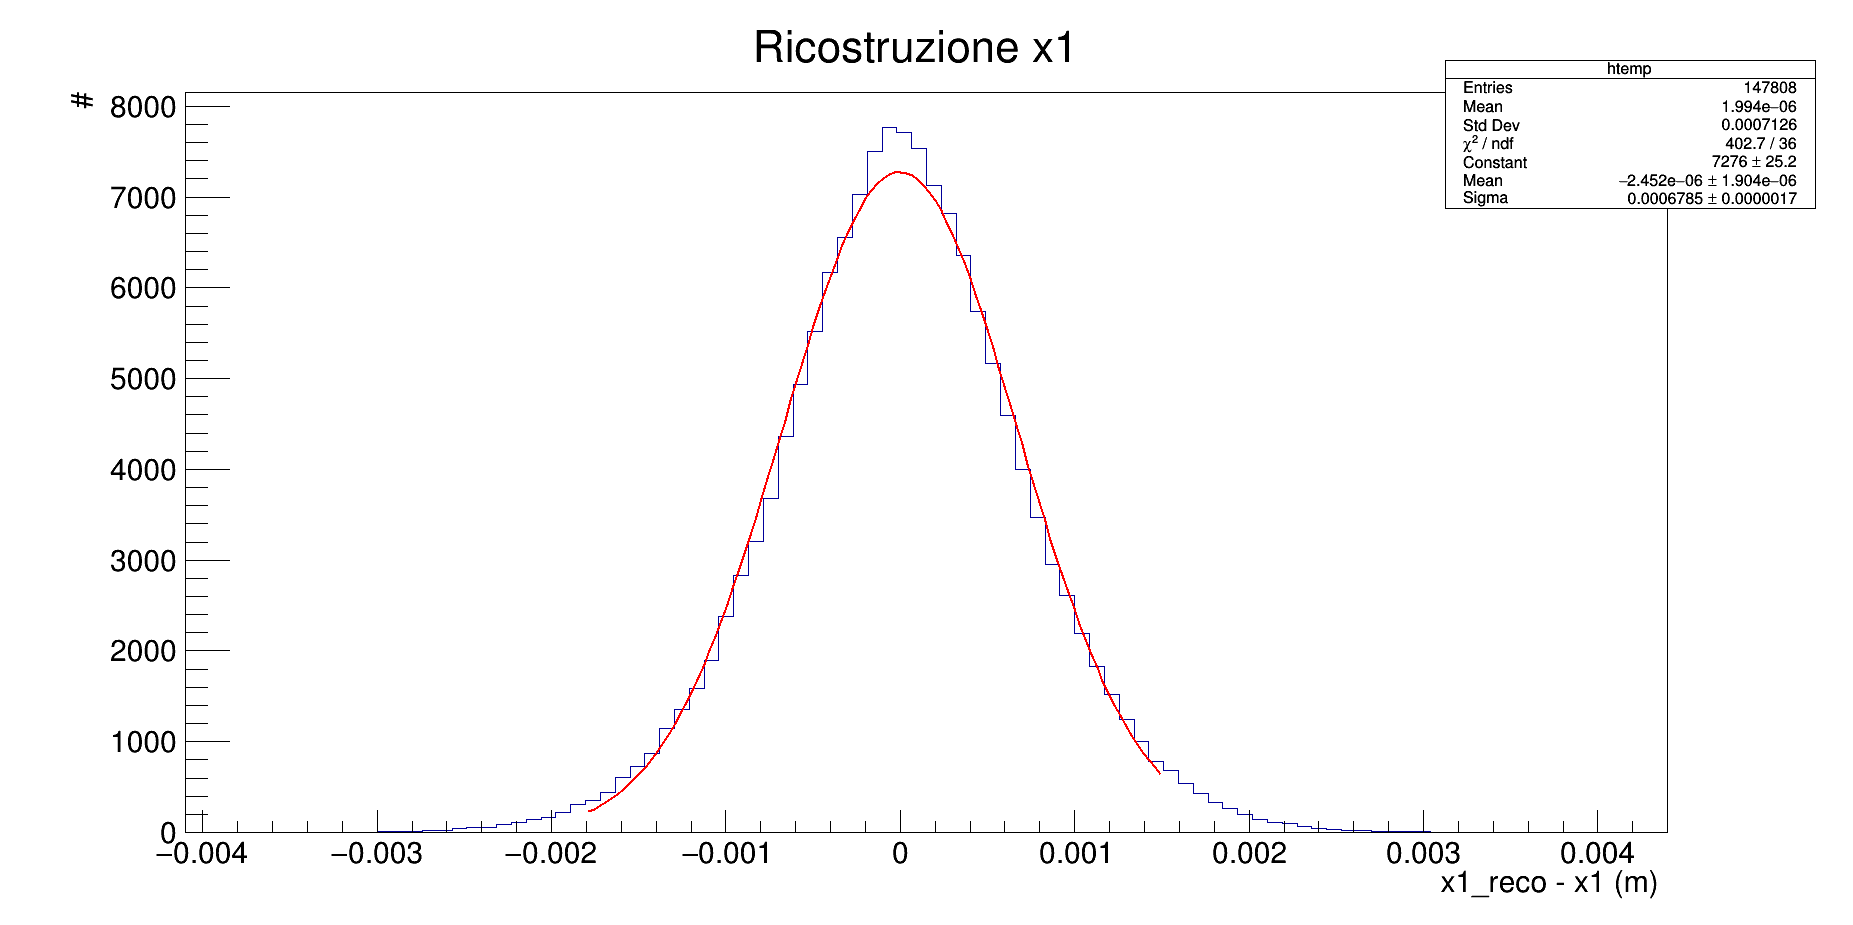
\includegraphics[scale=0.24]{reco_x1_N}
\caption{Risoluzione della coordinata x del rivelatore 1 nel decadimento a due corpi. In rosso, fit gaussiano (incompatibile).}
\label{fig:reco_x1_N}
\end{center}
\end{figure}

\clearpage

\begin{figure}[!h]
\begin{center}
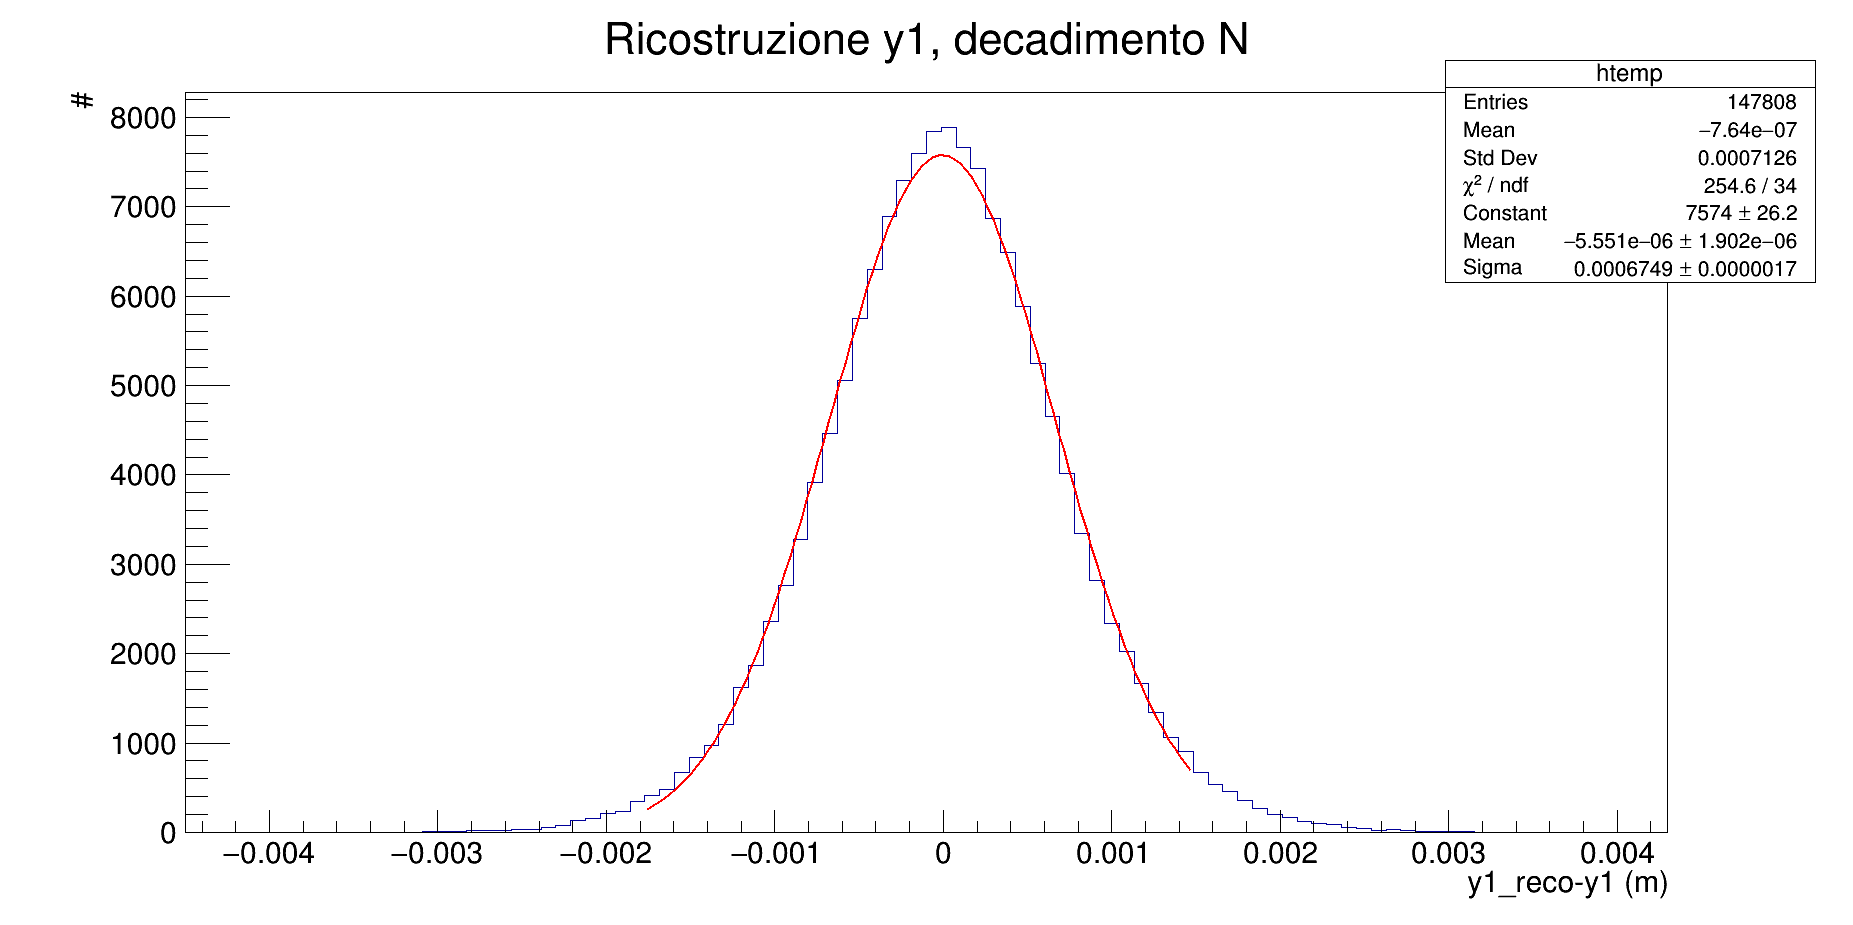
\includegraphics[scale=0.20]{reco_y1_N}
\caption{Risoluzione della coordinata y del rivelatore 1 nel decadimento a due corpi. In rosso, fit gaussiano (incompatibile).}
\label{fig:reco_y1_N}
\end{center}
\end{figure}

\begin{figure}[!h]
\begin{center}
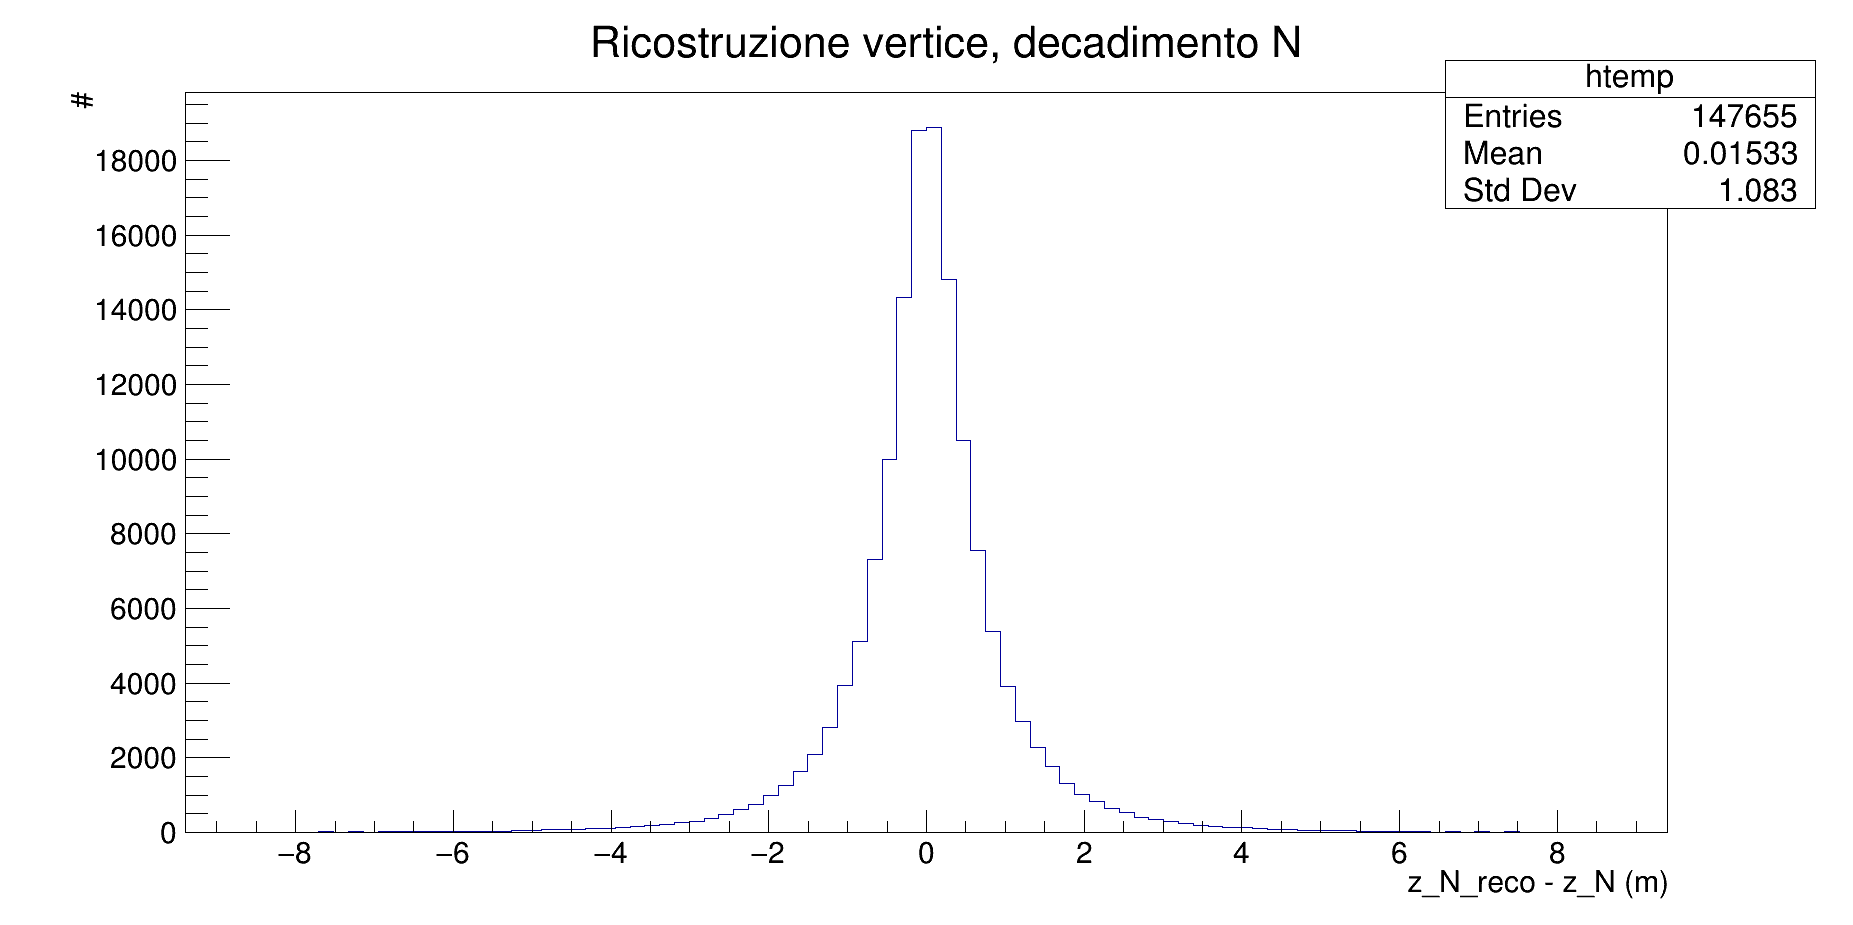
\includegraphics[scale=0.25]{reco_z_N}
\caption{Risoluzione della coordinata del vertice nel decadimento a due corpi.}
\label{fig:reco_z_N}
\end{center}
\end{figure}

\begin{figure}[!h]
\begin{center}
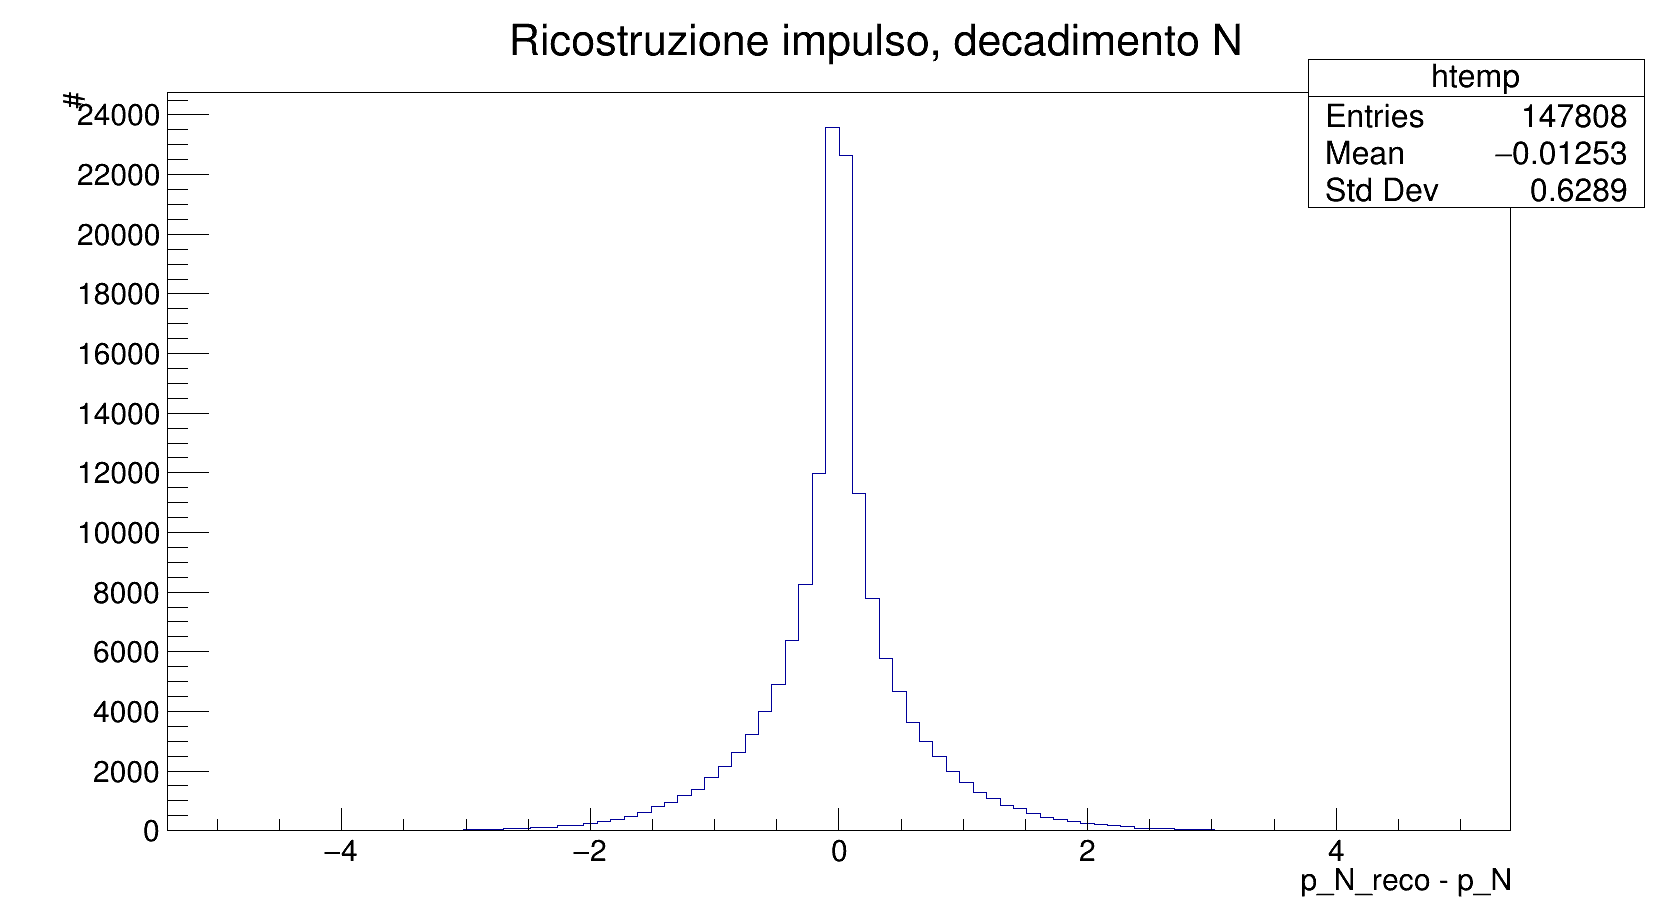
\includegraphics[scale=0.25]{reco_p_N}
\caption{Risoluzione dell'impulso nel decadimento a due corpi.}
\label{fig:reco_p_N}
\end{center}
\end{figure}


\begin{figure}[!h]
\begin{center}
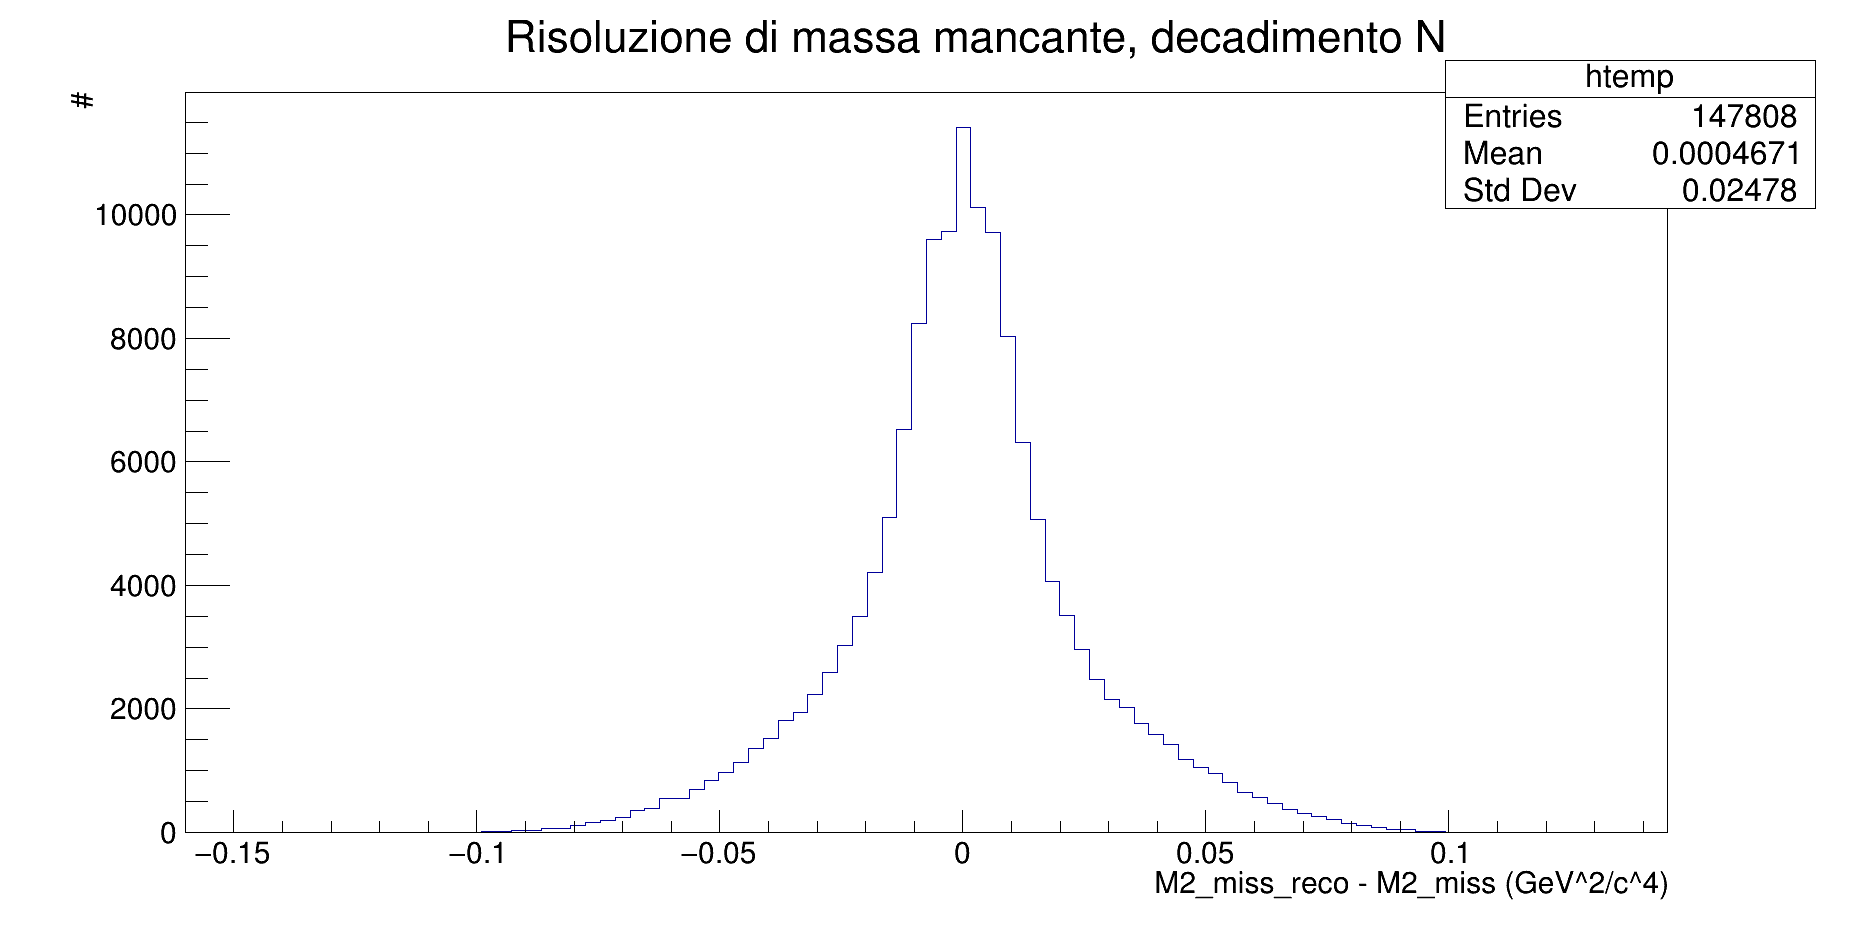
\includegraphics[scale=0.25]{reco_miss_N}
\caption{Risoluzione della massa mancante nel decadimento a due corpi.}
\label{fig:reco_miss_N}
\end{center}
\end{figure}

%%%%%%%%%%%%%%%%%%%%%

\begin{figure}[!h]
\begin{center}
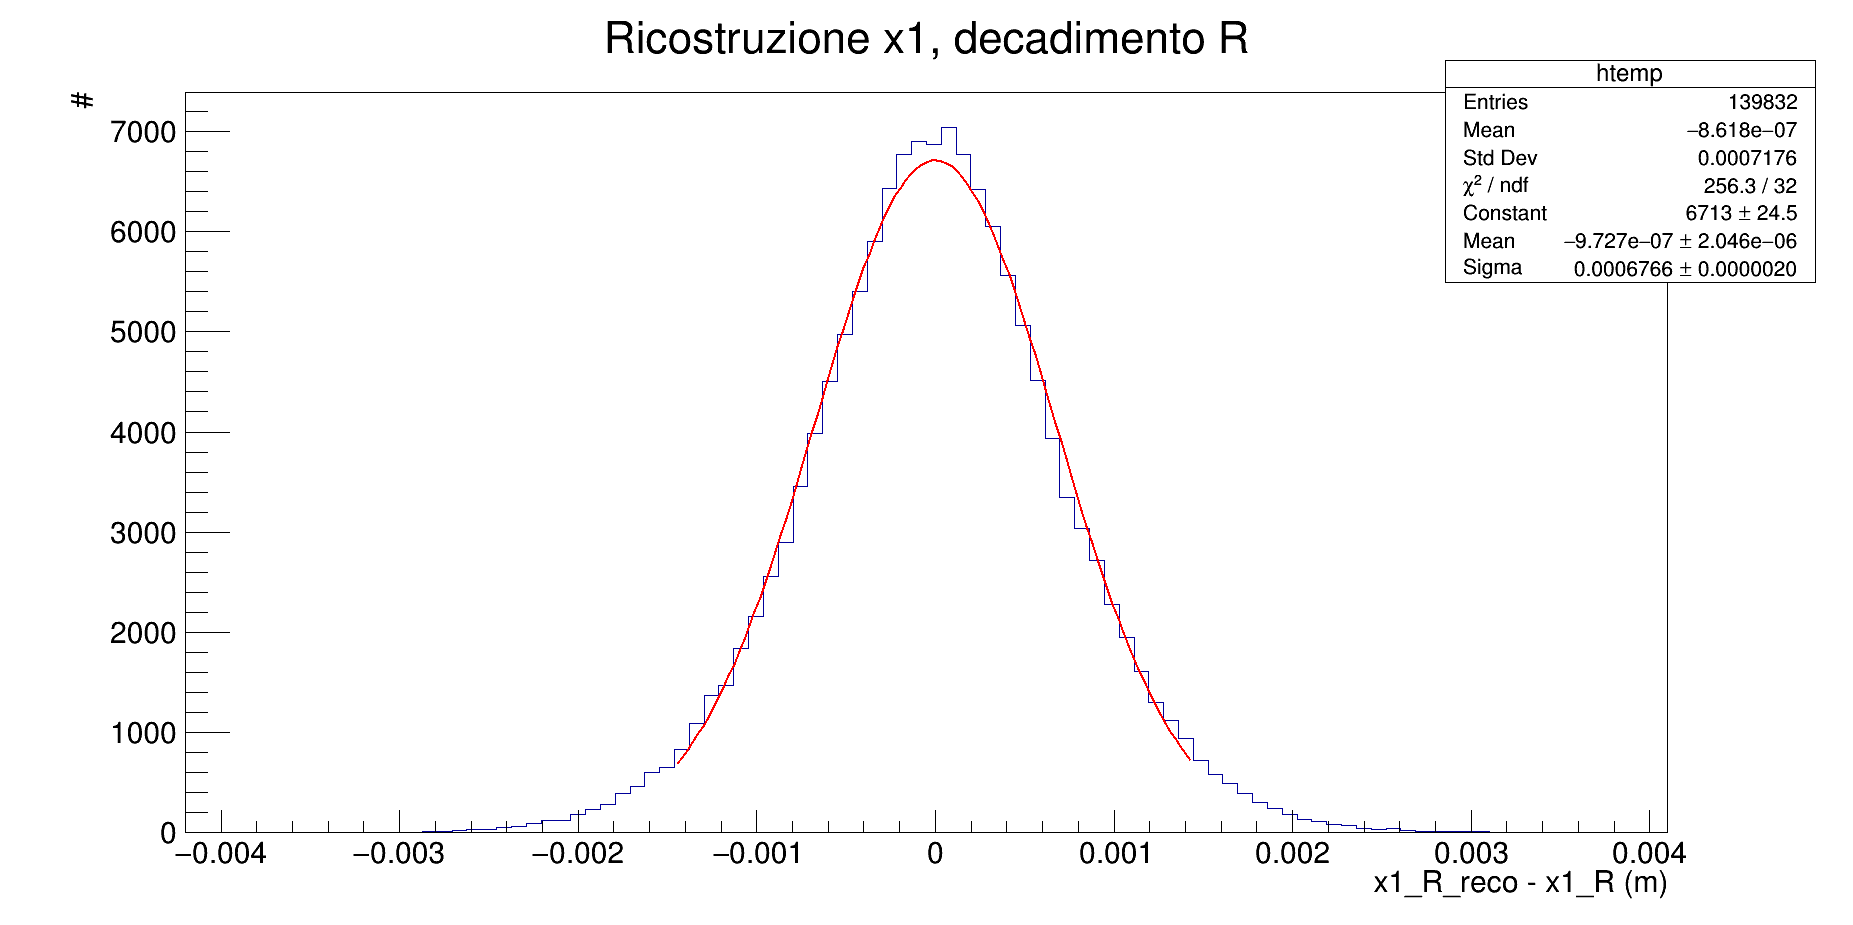
\includegraphics[scale=0.25]{reco_x1_R}
\caption{Risoluzione della coordinata x del rivelatore 1 nel decadimento a tre corpi. In rosso, fit gaussiano (incompatibile).}
\label{fig:reco_x1_R}
\end{center}
\end{figure}


\begin{figure}[!h]
\begin{center}
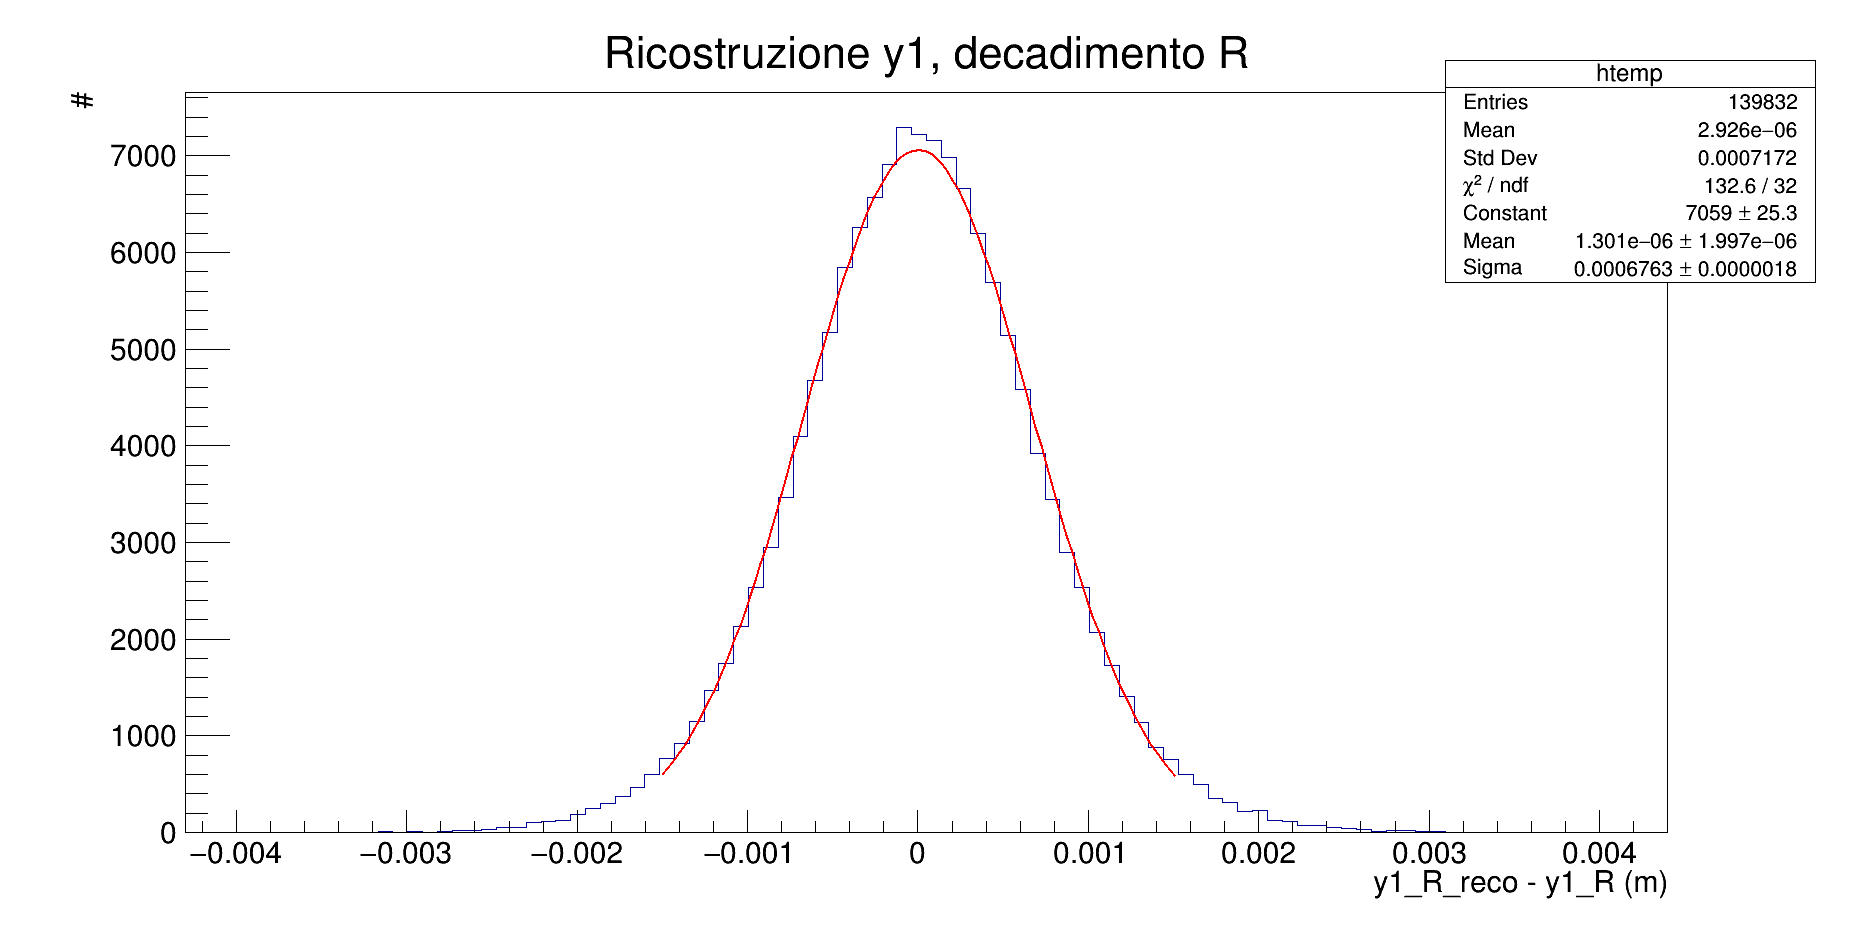
\includegraphics[scale=0.25]{reco_y1_R}
\caption{Risoluzione della coordinata y del rivelatore 1 nel decadimento a tre corpi. In rosso, fit gaussiano (incompatibile).}
\label{fig:reco_y1_R}
\end{center}
\end{figure}

\begin{figure}[!h]
\begin{center}
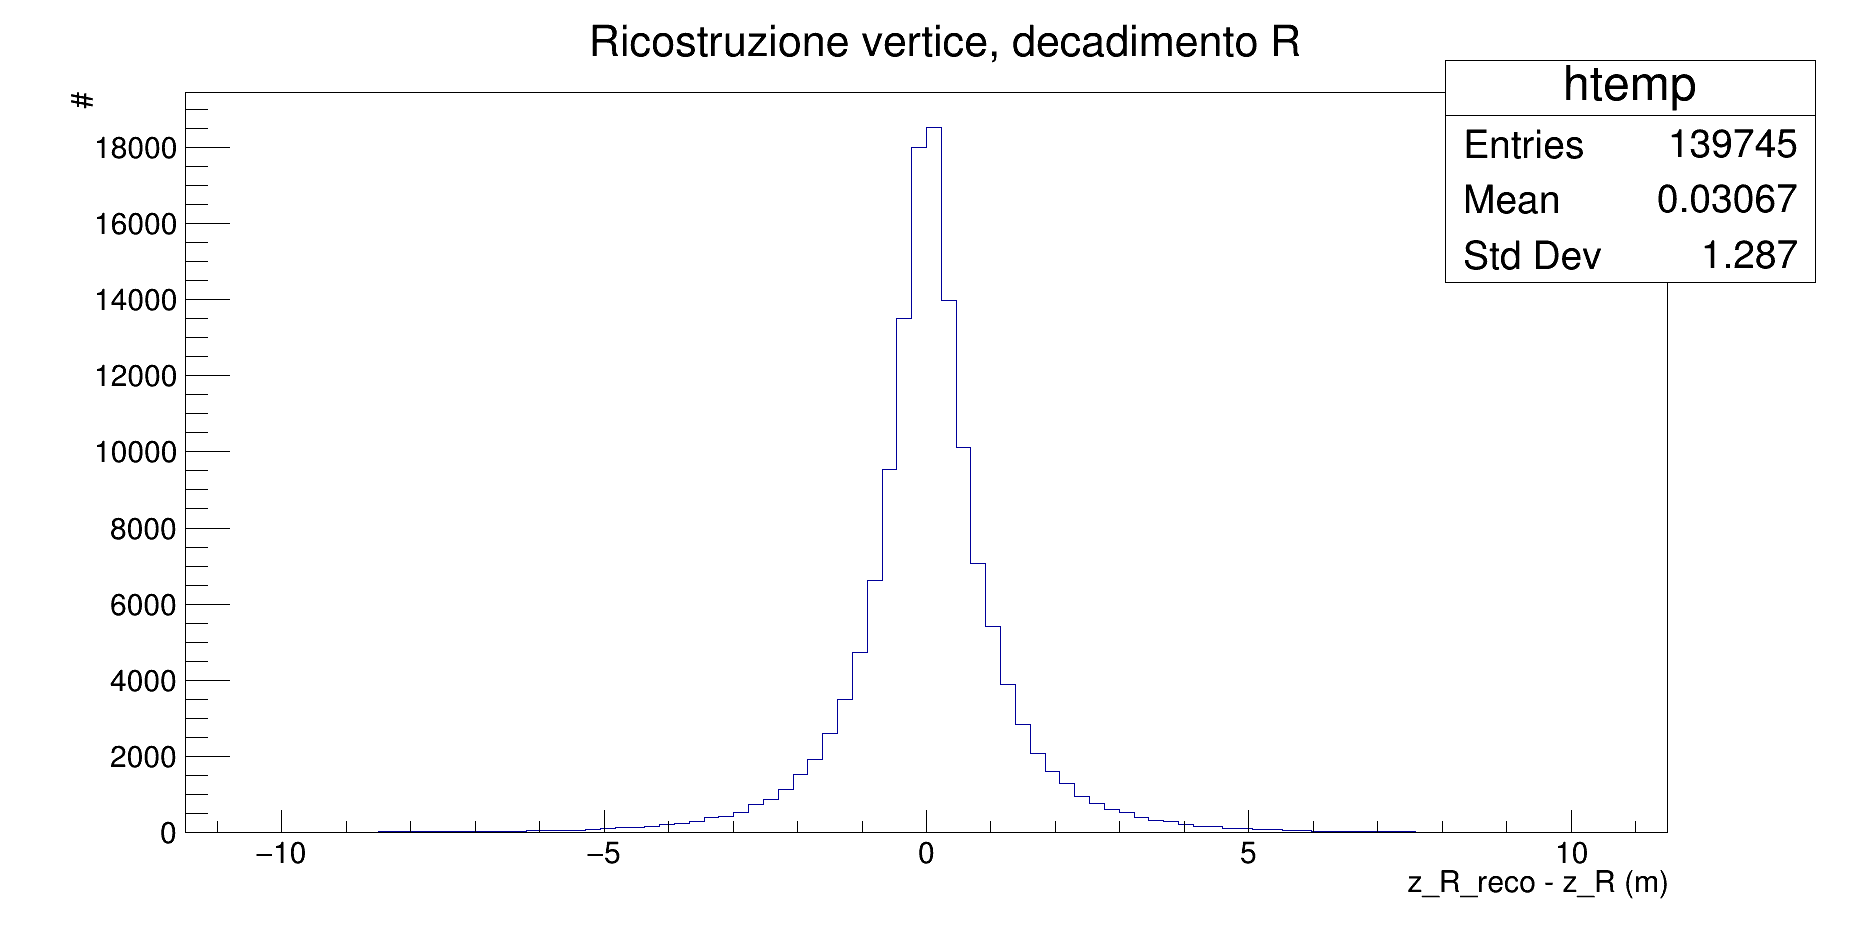
\includegraphics[scale=0.25]{reco_z_R}
\caption{Risoluzione della coordinata del vertice nel decadimento a tre corpi.}
\label{fig:reco_z_R}
\end{center}
\end{figure}


\begin{figure}[!h]
\begin{center}
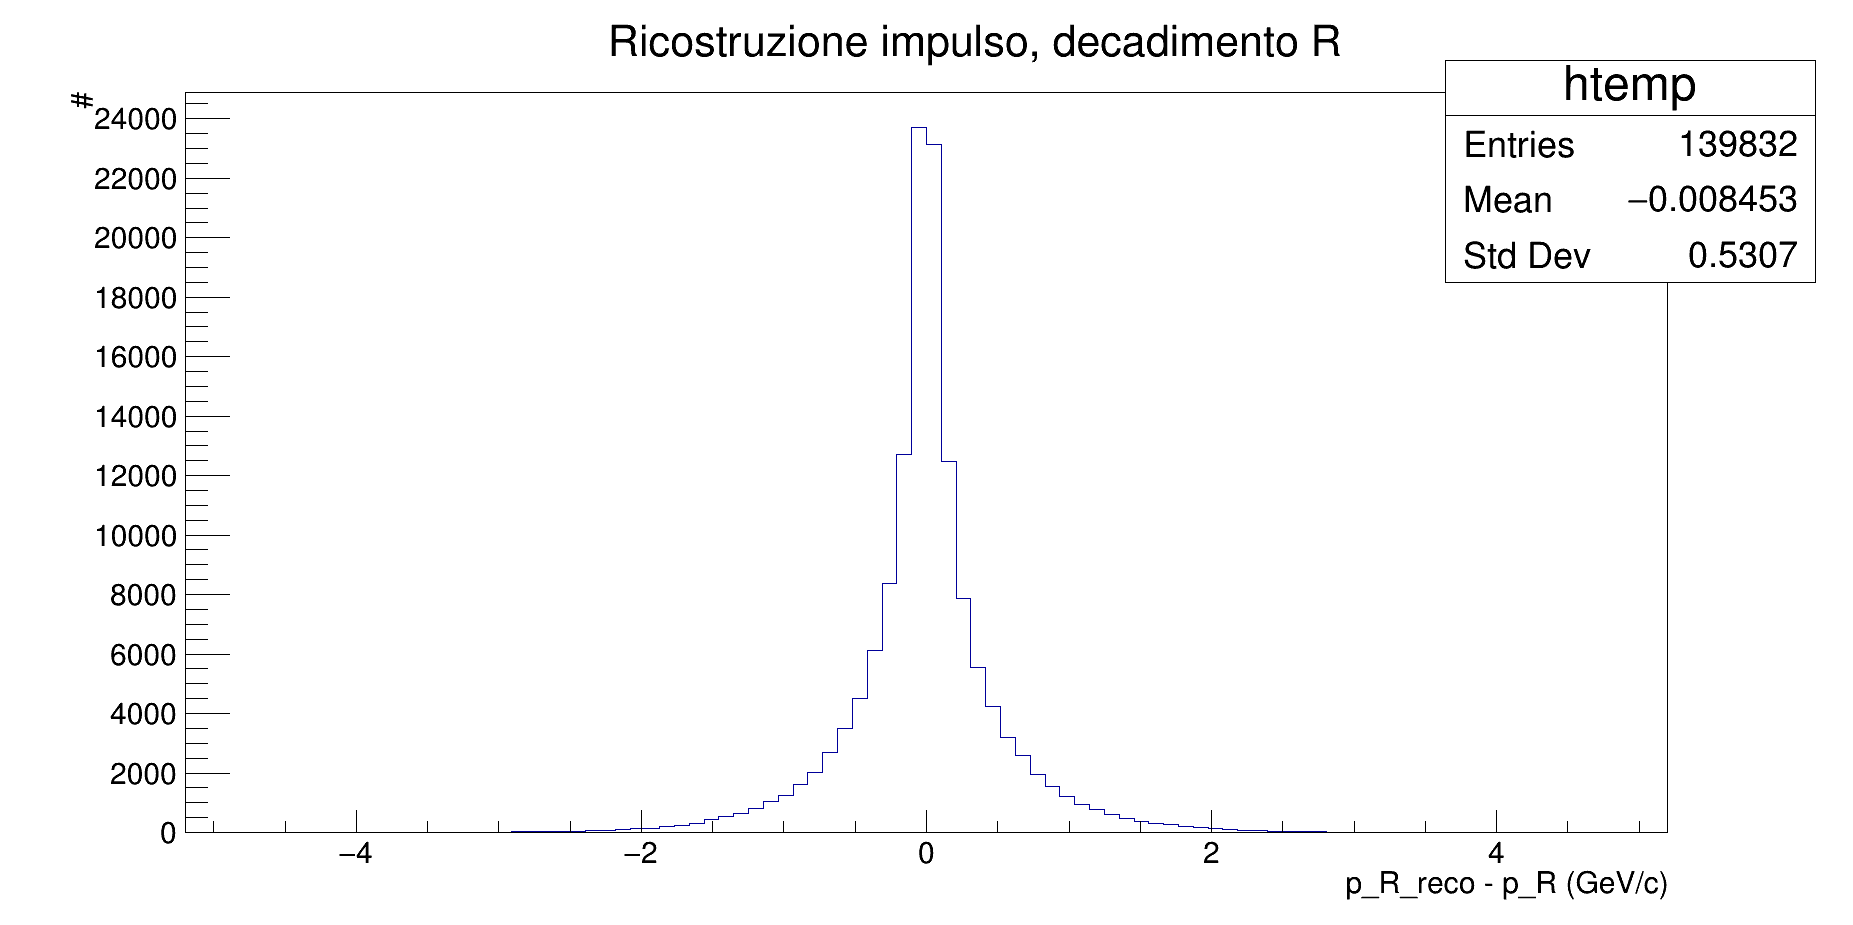
\includegraphics[scale=0.25]{reco_p_R}
\caption{Risoluzione dell'impulso nel decadimento a tre corpi.}
\label{fig:reco_p_R}
\end{center}
\end{figure}


\begin{figure}[!h]
\begin{center}
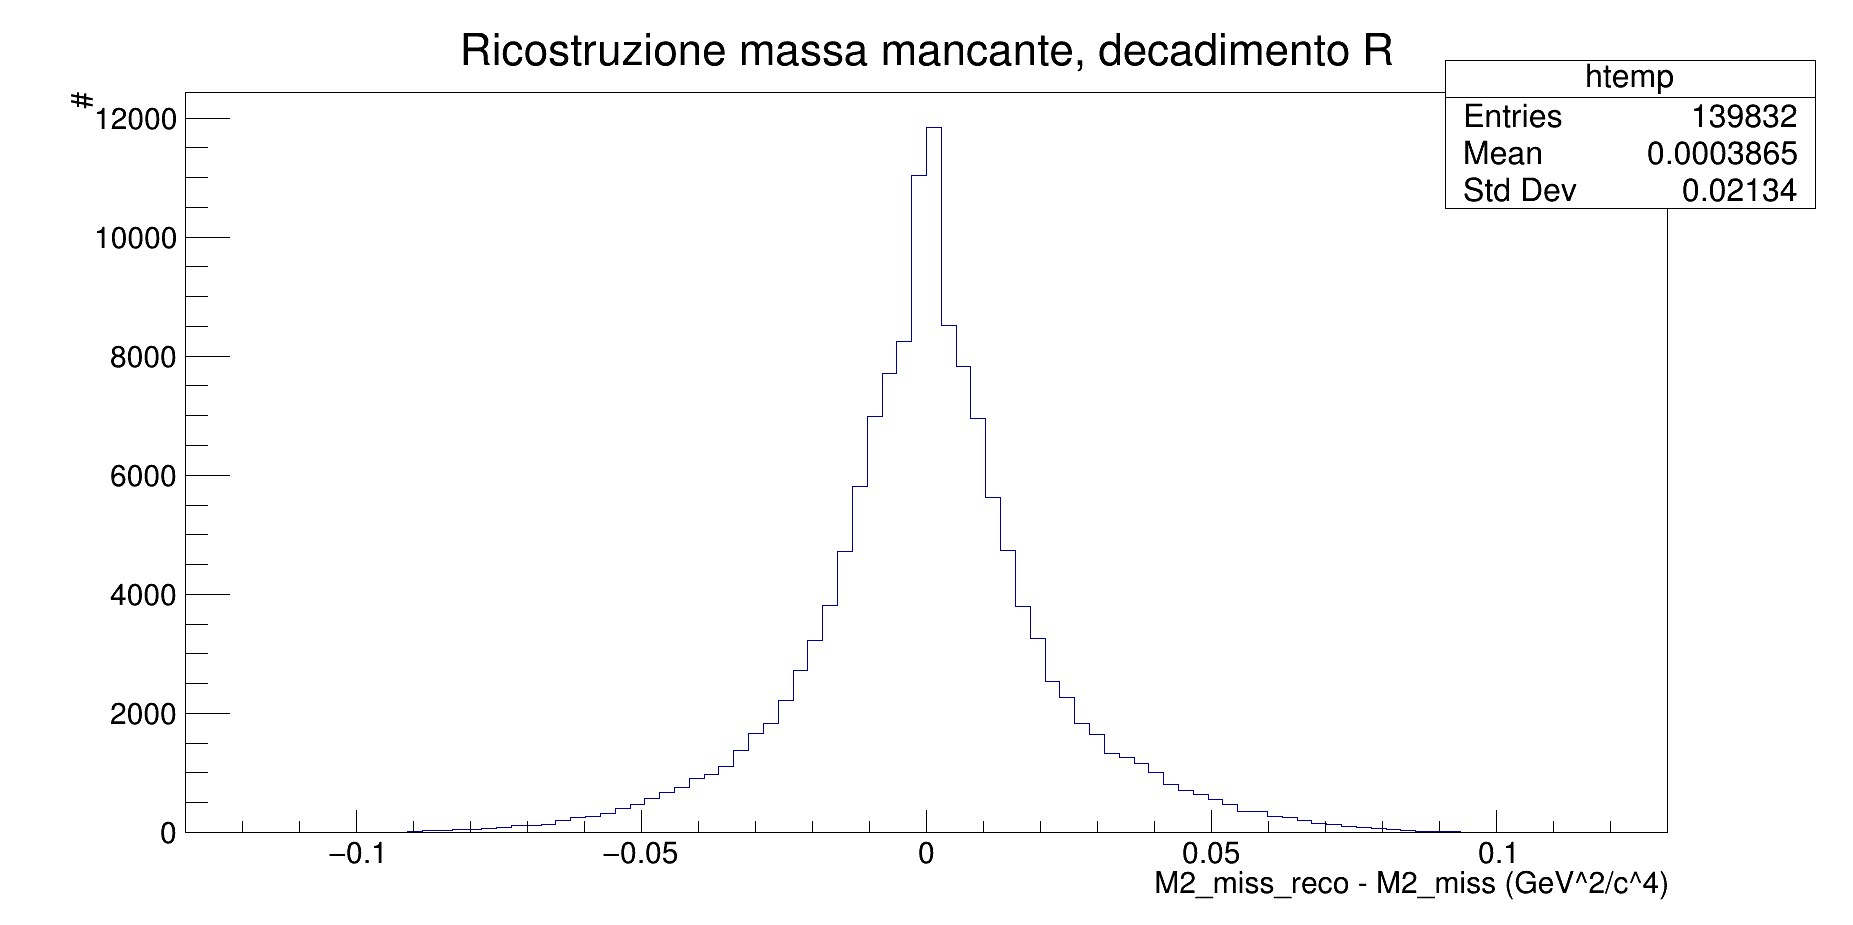
\includegraphics[scale=0.25]{reco_miss_R}
\caption{Risoluzione della massa mancante nel decadimento a tre corpi.}
\label{fig:reco_miss_R}
\end{center}
\end{figure}

%%%%%%%%%

\begin{figure}[!h]
\begin{center}
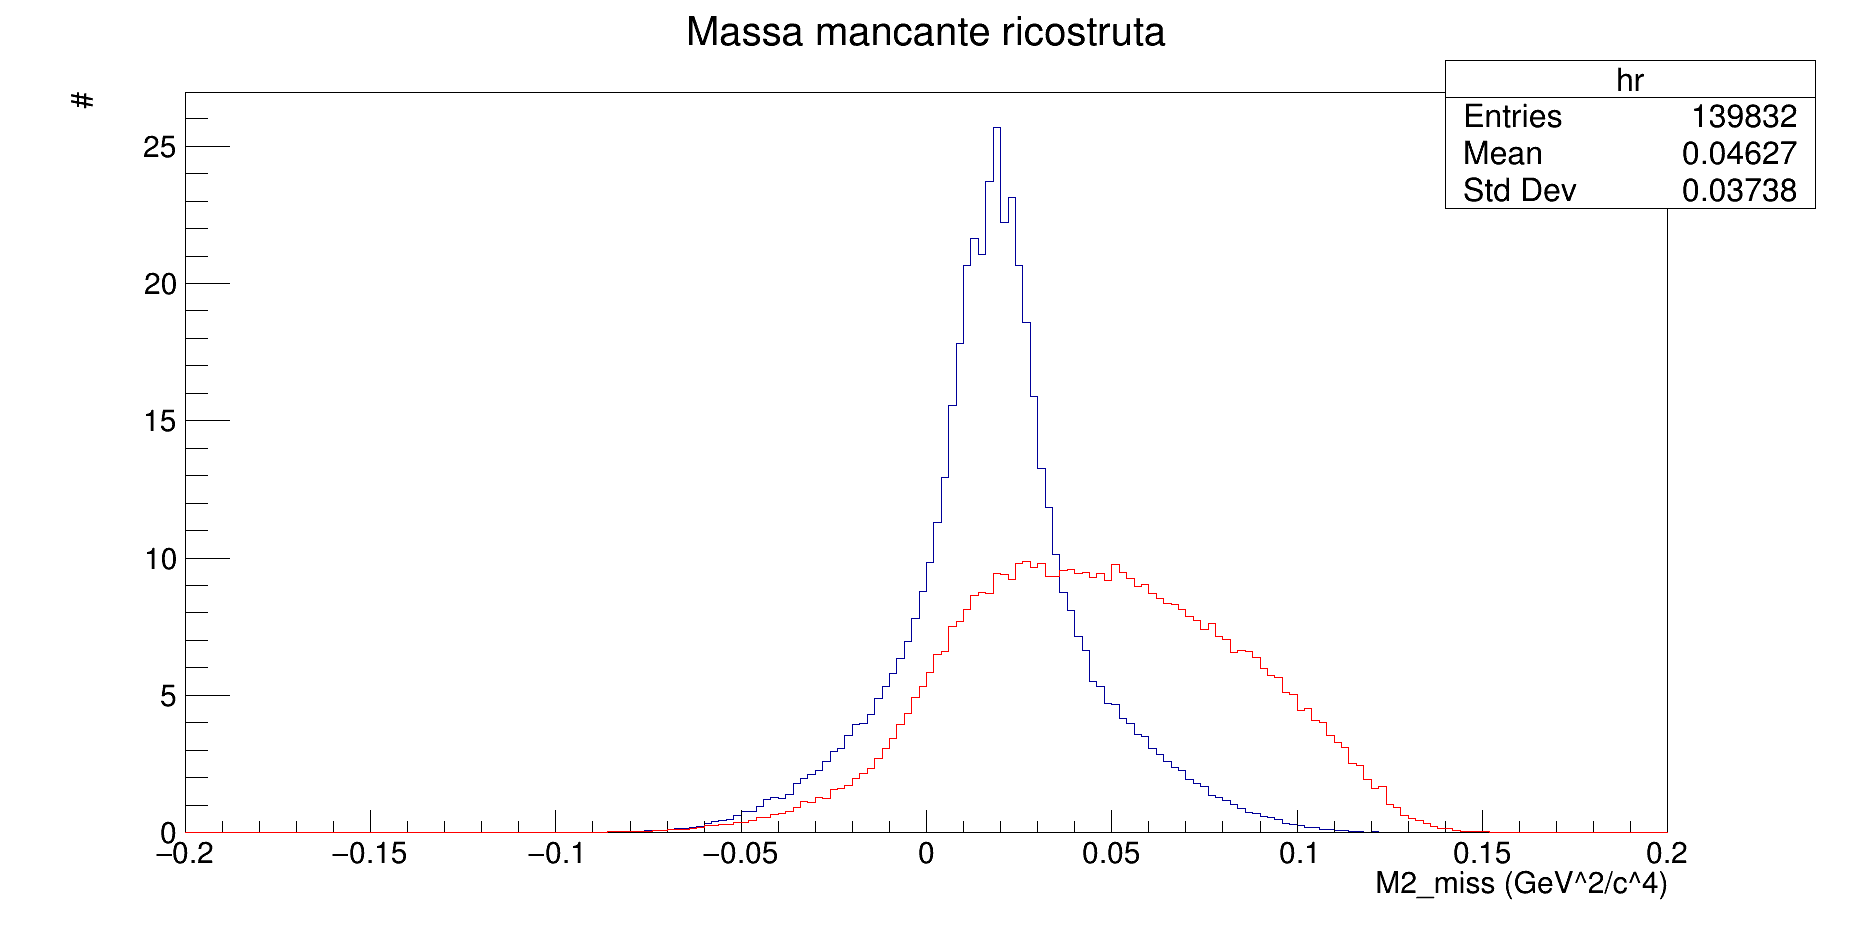
\includegraphics[scale=0.25]{reco_miss_norm}
\caption{Profilo di massa mancante ricostruito per i due canali di decadimento (rosso = tre corpi, blu = due corpi). Le distribuzioni
sono normalizzate.}
\label{fig:reco_miss_norm}
\end{center}
\end{figure}

\clearpage

\section{\ Appendice B: Calcolo dello stimatore del branching ratio} \label{sec:calcoli}
\justify

Supponiamo di usare un flusso continuo di $K^+$ con rate medio R e protrarre la misura per un tempo t. Il numero di decadimenti medi in un tempo t è: 

$$
\mu = Rt
$$

Ci chiediamo prima di tutto quale sia la distribuzione degli eventi che soddisfano il taglio, dato che sono stati accettati dalla geometria del sistema. La selezione è della forma $M^2_{miss} > M^2_c$, dove $M^2_{miss}$ è la massa mancante e $M^2_c$ il valore critico scelto per la selezione. La probabilità che $n$ eventi superino il taglio di massa mancante dato che $N_m$ sono passati attraverso l'apparato sperimentale è:
$$
P(n | N_m) = Bin(n | N_m, p_m)
$$

\begin{align*}
\begin{split}
& p_m = P(M^2_{miss} > M^2_c | (N\ mis \cup R\ mis) = \\
& \frac{P(M^2_{miss} > M^2_c\ |\ N\ mis)P(N\ mis\ |\ dec) + P(M^2_{miss} > M^2_c\ |\ R\ mis)P(R\ mis | R\ dec)}{P(N\ mis\ |\ dec) + P(R\ mis\ |\ dec)} = \\
& \frac{a_{N, cut}a_{N, geom}BR_N + a_{R, cut}a_{R, geom}BR_R}{a_{N, geom}BR_N + a_{R, geom}BR_R} \\
\end{split}
\end{align*}

\justify

dove \textit{N(R) mis} è l'evento \textit{``un $\pi^+$ proveniente dal decadimento a due(tre) corpi è stato misurato dall'apparato sperimentale''} e \textit{N(R) dec} è l'evento \textit{``un $\pi^+$ è decaduto nel canale a due(tre) corpi''}. $a$ sono invece le accettanze geometriche (geom) e di selezione (cut).

Supponiamo ora di fissare il numero di $K^+$ decaduti a $\mu$, che equivale a fissare il tempo di misura:

$$
P(n | \mu) = \sum_{N_m = n}^{\mu} P(n | N_m)P(N_m | \mu) = \sum_{N_m = n}^{\mu} Bin(n | N_m, p_m) Bin(N_m | \mu, p_d)
$$

$$
p_d = P(mis | dec) = P(N\ mis\ |\ dec) + P(R\ mis\ |\ dec) = a_{N,geom}BR_N + a_{R, geom}BR_R
$$

essendo la convoluzione di due binomiali ancora binomiale si ottiene: 

$$
P(n | \mu) = Bin(n | \mu, p_m p_d)
$$

Risulta quindi:

$$
E(n) = \mu (a_{N,cut}a_{N,geom}BR_N + a_{R,cut}a_{R,geom}BR_R)
$$
$$
Var(n) = E(n)(1 - a_{N,geom}BR_N - a_{R,cut}a_{R,geom}BR_R) \approx E(n)
$$

dove l'approssimazione è giustificata dal fatto che da un lato si cercherà di minimizzare l'accettanza del canale N, dall'altro perché $BR_R$ è molto piccolo.

Definiamo quindi la variabile aleatoria:
$$
n_R = n - \mu (a_{N,cut}a_{N,geom}BR_N)
$$

Che è sostanzialmente la stima del numero di eventi di segnale. 

$$
E(n_R) = \mu (a_{R,cut}a_{R,geom}BR_R) \rightarrow BR_R = \frac{E(n_R)}{\mu a_{R,cut}a_{R,geom}}
$$

Si può dunque definire lo stimatore:
$$
\widehat{BR_R} = \frac{n_R}{\mu (a_{R,cut}a_{R,geom})}
$$
$$
E(\widehat{BR_R}) = BR_R
$$
$$
Var(\widehat{BR_R}) = \frac{1}{\mu} \frac{a_{N,cut}a_{N,geom}BR_N + a_{R,cut}a_{R,geom}BR_R}{(a_{R,cut}a_{R,geom})^2}
$$

dove la quantità $\mu \cdot Var(\widehat{BR_R})$ è ricavabile dalla simulazione e non dipende dal tempo.

Fissata la precisione che si vuole raggiungere al valore $\alpha$, si può stimare il tempo di misura necessario: 
$$
\frac{Var(\widehat{BR_R})}{BR_R^2} = \alpha^2 \rightarrow t = \frac{1}{R \alpha^2 BR_R^2} (\mu \cdot Var(\widehat{BR_R}))
$$

\section{\ Appendice C: Valori delle costanti e unità di misura}

\begin{itemize}
\item $c = 299792458\ m/s$
\item $M_K = 493.677\ MeV/c^2$
\item $M_{\pi^{+}} = 139.57018\ MeV/c^2$
\item $M_{\pi^0} = 134.9766\ MeV/c^2$
\item $\tau = 1.238\cdot 10^{-8}\ s$
\item $\tau_\pi = 2.6\cdot 10^{-8}\ s$
\end{itemize}

Le unità di misura, laddove non indicate, sono da intendersi \textit{m} per le lunghezze, \textit{GeV} per le energie, \textit{GeV/c} per gli impulsi, \textit{$GeV/c^2$} per le masse, \textit{s} per i tempi.

\newpage

\input{bibRareDecay.bib}

\end{document}

